%\documentclass{aastex}
\documentclass[iop]{emulateapj}
\usepackage[utf8]{inputenc}
\usepackage{apjfonts}
\usepackage{multirow}

\usepackage{graphicx}
\usepackage{epstopdf}

\newcommand{\myshorttitle}{Near-IR Imaging of M31}
\newcommand{\myshortauthors}{Sick et al.}

\usepackage{color}
\usepackage[dvipsnames]{xcolor}
\usepackage[pdfauthor={\myshortauthors},pdftitle={\myshorttitle},colorlinks=true,citecolor=blue,linkcolor=blue,urlcolor=blue]{hyperref}
\usepackage{url}

\usepackage{amssymb}
\usepackage{amsmath}

\usepackage{natbib}
\bibliographystyle{apj}

\newcommand{\ie}{\textit{i.e.,~}}
\newcommand{\eg}{\textit{e.g.,~}}
\newcommand{\etal}{et~al~}
\newcommand{\vect}[1]{\boldsymbol{#1}} % vectors or images
\newcommand{\sw}[1]{\textit{#1}} % style software titles
\newcommand{\sn}{\ensuremath{S/N}} % signal to noise
\newcommand{\sersic}{S\'{e}rsic}
\newcommand{\iiwione}{\sw{`I`iwi 1.0}}
\newcommand{\androids}{\textsc{androids}}
\newcommand{\changeit}[1]{\textcolor{BrickRed}{\underline{#1}}} % markup bad sections
\newcommand{\todo}[1]{\textcolor{BurntOrange}{\textsf{#1}}} % markup TODOs
\newcommand{\comment}[1]{\textcolor{OliveGreen}{\textit{#1}}} % markup TODOs
\newcommand{\Fig}[1]{Fig.~\ref{fig:#1}}  % figure reference macro
\newcommand{\Eq}[1]{Eq.~\ref{eq:#1}}  % equation reference macro
\newcommand{\Tab}[1]{Table~\ref{tab:#1}}  % table reference macro
\newcommand{\Sec}[1]{\S\ref{sec:#1}}  % section reference macro

% To track draft versions in git
\IfFileExists{vc.tex}{\input{vc}}{}

% aastex setup
\shorttitle{\myshorttitle}
\shortauthors{\myshortauthors}

\begin{document}
    \IfFileExists{vc.tex}{\slugcomment{Version \VCRevision\ by \VCAuthor\ on \VCDateTEX , \VCTime.}
}{\slugcomment{Revision unknown.}}
\title{ANDROIDS I. Near-Infrared Imaging of M31}
\author{Jonathan Sick, Stéphane Courteau}
\affil{Queen's University}
\email{jsick@astro.queensu.ca}
\author{Jean-Charles Cuillandre}
\affil{Canada-France Hawaii Telescope Corp.}
\author{Michael McDonald}
\affil{Massachusetts Institute of Technology}
\author{Brent Tully}
\affil{University of Hawaii Institute for Astronomy}
\and
\author{The \androids\ collaboration}
\affil{}

% ============================================================================
\begin{abstract}
\comment{PROVISIONAL}.
We present near-infrared $J$ and $K_s$ images of the Andromeda Galaxy made with WIRCam on the Canada-France-Hawaii Telescope.
These images provide the highest resolution of M31's entire bulge and disk (within $R=22$~kpc) to date, simultaneously resolving stars and recovering M31's near-infrared surface brightness.
This work extensively develops and tests our WIRCam calibrations, which are complicated by the brightness of near-infrared sky glow (which is 3 dex brighter than M31's disk at $R=20$~kpc), spatiotemporal variations in the sky glow and instrumental calibrations, and by the exceptionally large area of the M31 disk that we survey.
We find that WIRCam data should be calibrated with real-time sky flats, to overcome flat field variability of order 1\% over 20 minutes.
Two sky-target nodding strategies were tested, and we find that strictly minimizing sky sampling latency does not maximize sky subtraction accuracy, which is at best 1\% of certainty.
Instead, our final surface brightness calibration relies upon solving for sky offsets, nudges of flux to each WIRCam image, that reduce image-to-image differences.
Sky offset optimizations reduce image-to-image residuals  to 0.02\% of the sky brightness.
Monte Carlo simulations show that the absolute surface brightness level of the disk at $R=15$~kpc is uncertain by \todo{TODO}, necessitating independent surface brightness calibration based on resolved stellar populations.
\todo{ADD SCIENCE CONTEXT? ADD DISCUSSION OF SHAPE VARIABILITY.}
\end{abstract}

% ============================================================================
\section{Introduction}
\label{sec:intro}

Near-infrared (NIR) light provides a valuable view into galaxies.
The NIR is a segment of the spectral energy distribution (SED) that is only recently gaining attention in galaxy studies, mostly due to the immaturity of detectors.
In conjunction with ultraviolet and optical bands, the NIR offers a partial remedy for the age-metallicity-dust degeneracy that plague stellar population interpretations. 
Traditionally the NIR has also been treated as a stellar mass map, tracing the low end of the stellar initial mass function with minimal dust obfuscation.
Yet the scientific promise of the near-infrared as not been realized.

\cite{Maraston:1998} pointed out that most of the NIR light from intermediate age populations is contributed by thermally-pulsating asymptotic giant branch stars (TP-AGBs).
These TP-AGB stars are notoriously difficult to model and include in spectral synthesis models.
As a result, the optical-NIR SEDs of galaxies cannot be consistently modelled \citep{Taylor:2011}.
Consequently, the best practise for stellar mass estimation as advocated by \cite{Taylor:2011} is to omit the NIR SED from fits, and rely upon useful stellar population degeneracies that, by coincidence, enforce a $g-i$~vs.~$\Upsilon_*$ relation.

One means forward for NIR is improved empirical spectral libraries. 
\todo{Cite X-shooter, other NIR spectral library efforts?}
Another way to understand, and possibly calibrate, the NIR light is to observe nearby galaxies where stellar populations can be robustly understood (with exhaustive SED coverage and resolved stellar populations).
Here the Andromeda galaxy stands as a unique and important target.
It is visible to the Northern Hemisphere and thus to the premiere wide-field NIR imager (CFHT/WIRCam), and close enough (785~kpc) that stars can be resolved throughout the disk without adaptive optics.

\cite{Beaton:2007} assembled a 2.8\arcdeg\ $JHK_s$ mosaic centered on M31 with the 2MASS 6X program.
Those observations, which trace the stellar galaxy mass, were used by \cite{Athanassoula:2006} as evidence of a bar embedded in a classical bulge.
But beyond the bulge, the 2MASS 6X images have limited utility.
\cite{Courteau:2011} find sky uncertainty prevents using the 2MASS 6X to infer structural and photometric properties of the disk.
Further, the pixel scale of 1\arcsec\ and integration depth of 46.8 seconds prevents point source measurements of the 2MASS 6X images.
As a result, the de facto state-of-the-art NIR view of M31 is the slightly longer 3.6 $\mu$m Spitzer/IRAC map of \cite{Barmby:2006}.
Spitzer obviates the issue of sky estimation, although the pixel scale of 0\farcs86 also prevents point source measurements of individual stars in the M31 disk.

In this paper, we present a survey of the M31 bulge and disk with CFHT/WIRCam in the $J$ and $K_s$ bands.
These are the first global near-infrared observations of M31 that simultaneously resolve throughout the mid- and outer-disk, while also recovering attempting to rigorously recover the NIR surface brightness.
While future contributions will explore the resolved near-IR stellar populations, our focus here is the surface brightness calibration of the WIRCam data set, and exploration of NIR sky subtraction uncertainties.
Section~\ref{sec:Observations} describes the novel observational strategies used to reduce sky subtraction uncertainties.
Section~\ref{sec:reduction} describes the image reduction pipeline; a particularly important aspect of this is night sky flat fielding (\S\ref{sec:flats}).
In \S\ref{sec:scalar} we present our method for recovering the galaxy surface brightness by minimizing the image-to-image differences across the mosaic.
We estimate the systematic uncertainties in our mosaic solution in \S\ref{sec:systematics}, where we also compare our technique to the Montage package \citep{Berriman:2008} and the Spitzer/IRAC mosaics.
Finally in \S\ref{sec:conclusions} we summarize the uncertainty of NIR sky subtraction on the scale of M31.

\section{Observations}
\label{sec:Observations}

\begin{figure}[t]
	\centering
		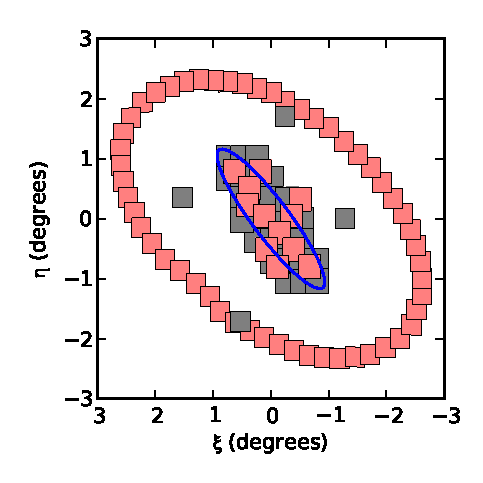
\includegraphics[width=3in]{figs/fieldmap}
	\caption{WIRCam field positions on M31. Grey fields at center at the 27 disk fields observed in 2007B, surrounded by 4 sky fields. Red fields at center are the 12 disk fields observed in 2007B. The red ring of 53 fields is the 2009B sky sampling ring. The blue ellipse marks the M31 disk at $R=20$ kpc along the major axis. Coordinates are centered on the nucleus of M31 with North up, and East towards left.}
	\label{fig:fieldmap}
	% made with skyoffsets/chart.py
    % TODO fix colouring of disk vs sky fields.
\end{figure}

% Surface brightness CI from skyoffset/net_sky_level.py
% Median and 95% C.I.
% 2007B J 15.1195176911 ; 14.9139114767 -- 15.3477818651
% 2009B J dim 14.5613758489 ; 14.2933487068 -- 14.8544020768
% 2009B J bright 15.2006801085 ; 15.1336648803 -- 15.2789519627
% 2007B Ks 13.354737759 ; 13.1811645305 -- 13.6149313145
% 2009B Ks 13.27306929 ; 13.1173594814 -- 13.4222534742

\begin{table*}[t]
    \caption[Summary of WIRCam observing programs]{Summary of WIRCam observing programs. ST Nods are coded with superscripts to denote the number of times an observation is repeated at a given field. Efficiency (Eff.) is the percentage of time in a program allocated to integrating the disk of M31, compared from nodding, read out and sky overheads. Seeing is measured from stars in sky images.}
    \label{tab:obssummary}
    
    \centering
    \begin{tabular}{lllllllllll}
        & & & & $\frac{T_\mathrm{int}}{\mathrm{field}}$ & $T_\mathrm{exp}$ & Eff. & $\mu_\mathrm{sky}$ 95\% C.I. & \multicolumn{3}{c}{PSF FWHM (arcsec)} \\ \cline{9-11}
    Semester & Band & $N_\mathrm{disk}$ & ST Nods & (min) &  (s) &  (\%) & (mag/arcsec$^2$) & 25th  & 50th & 75th \\
    \hline
    \multirow{2}{*}{2007B} & $J$ & \multirow{2}{*}{27} & [S$^3$T$^8$S$^3$]$^{2}$S$^3$ & 12.5 & 47 & 49 & (14.9, 15.3) & 0.68 & 0.75 & 0.84 \\
     & $K_s$ &  & [S$^5$T$^{13}$S$^5$]${^2}$S$^5$ & 10.8 & 25 & 42 & (13.2, 13.6) & 0.60 &  0.65 & 0.73 \\
     \hline
     \multirow{2}{*}{2009B} & $J$ & \multirow{2}{*}{12} & \multirow{2}{*}{[ST$^2$S]$^{20}$S} & \multirow{2}{*}{13.3} & \multirow{2}{*}{20} & \multirow{2}{*}{26} & (14.3, 14.6), (15.1, 15.3) & 0.61 & 0.69 & 0.83 \\
      & $K_s$ & & & & & & (13.1, 13.4) & 0.60 & 0.66 & 0.76 \\
    \end{tabular}
\end{table*}

% \begin{deluxetable}{10}
% % \tabletypesize{\small} % or \footnotesize or \scriptsize
% % \rotate
% % \tablewidth{⟨dimen ⟩}
% % \tablenum{⟨text ⟩}
% \tablecolumns{⟨num ⟩}
% \tablecaption{Summary of WIRCam observing programs. Efficiency (Eff.) is the percentage of time in a program allocated to integrating the disk of M31, compared from nodding, read out and sky overheads. Seeing is measured from stars in sky images.
%     \label{⟨key ⟩}}
% \tablehead{⟨text ⟩}
% \end{deluxetable}

The Andromeda Galaxy (M31) was observed in the NIR using the WIRCam instrument, mounted to the 3.6-meter Canada-France-Hawaii Telescope (CFHT), at the summit of Mauna Kea in Hawaii. Observations were carried out exclusively in the NIR $J$ ($\lambda_0 \sim 1.2 \mu\mathrm{m}$) and $K_s$ ($\lambda_0 \sim 2.2 \mu\mathrm{m}$) bands.

WIRCam itself is an array of four HgCdTe HAWAII-RG2 detectors \citep{Puget:2004}.
Each detector comprises $2048\times 2048$ pixels, with a scale of 0\farcs 3. This pixel scale critically samples the typical seeing of 0\farcs 65~seen by CFHT\@.
For reference, $1\arcsec = 3.7~\mathrm{pc}$ across the disk of M31.
The detectors are arranged in a $2\times 2$ grid with 45\arcsec~gaps, so that the entire instrument covers $21.5\arcmin \times 21.5\arcmin$ of sky. It is truly the recent advent of NIR focal plane arrays, like WIRCam, that have enabled relatively efficient studies of M31 in the NIR.

The \androids\ WIRCam survey is designed to simultaneously resolve stars and recover the integrated surface brightness of the M31 disk. While the former objective is attained by requesting good seeing in Queued Service Observing mode (see \Tab{obssummary}), WIRCam has not previously been used to recover surface brightness at the accuracy required---$\mu_{K_s}\lesssim~22$~mag~arcsec$^{-2}$---across entire detector fields. As discussed in \Sec{intro}, NIR observations require frequent monitoring of the sky background. Since M31, with a $190\arcmin \times 60\arcmin$ optical disk, is much larger than the WIRCam fields of view, monitoring of the sky zeropoint is only possible by periodically pointing the telescope away from M31, towards blank sky---\emph{sky-target} (ST) nodding. 

Observations were taken over two semesters, 2007B and 2009B. The two campaigns employed different observing schemes, particularly sky-target nodding strategies. The reader is encouraged to regard these observational designs as \emph{hypotheses} for how to best conduct a wide-field surface brightness survey in the near-infrared from the ground. An objective of this paper is to discriminate between the virtues of the 2007B and 2009B programmes, and determine if observational design can improve the construction of a wide-field NIR mosaic.

\begin{figure}[t]
    \centering
        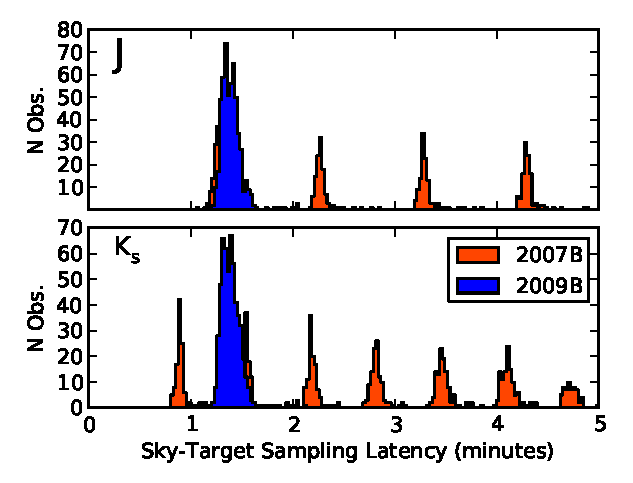
\includegraphics[width=3in]{figs/sky_target_lag}
    \caption{Time latency between target observations and sky field sampling in the 2007B and 2009B WIRCam observing runs. The 2009B program was designed to ensure that no disk sample would be removed by more than 1.5 minutes from a sky sample by using a STTS nodding pattern.}
    \label{fig:sky_target_lag}
    % made with skyoffsets/obs_run_stats.py
\end{figure}

\begin{figure}[t]
    \centering
        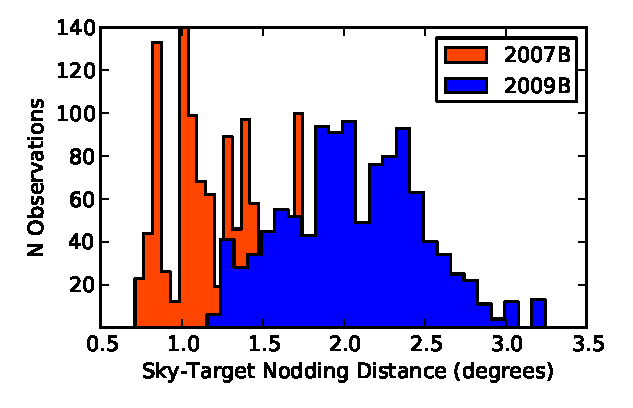
\includegraphics[width=3in]{figs/sky_target_dist}
    \caption{Distance between sky and target observations in the 2007B and 2009B WIRCam observing runs. The larger nodding distance of 2009B is a consequence of sky ring sampling. The maximum nodding distance across the sky ring was purposefully set to $\sim 3$\arcdeg\ to avoid excessive time overheads. As such, a given disk field only samples roughly of the full sky ring.}
    \label{fig:sky_target_dist}
    % made with skyoffsets/obs_run_stats.py
\end{figure}

\begin{figure}[t]
    \centering
        \includegraphics[width=3.25in]{figs/sky_level_hist}
    \caption{Sky levels observed in the 2007B (red outline) and 2009B (grey filled) programs.}
    \label{fig:net_sky_level}
    % made with skyoffset/net_sky_level.py
\end{figure}

\subsection{2007B Semester} % (fold)
\label{sec:obs7}

The initial survey was carried out in the 2007B semester by the CFHT Queue Service Observing under photometric conditions. This programme covers M31 with 27 contiguous WIRCam fields covering the entirety of M31 out to the optical radius: $\mu_V=23$ mag arcsec$^{-2}$, $R=20$~kpc. The fields are arranged with at least 1\arcmin\ overlap in declination, and approximately 5\arcmin\ overlap in right ascension.
% FIXME check overlaps
This arrangement yields a continuous mosaic that avoids masked pixels that obscure the eastern 3\arcmin\ of the WIRCam array. The field configuration is shown in \Fig{fieldmap}.

Each field was integrated for $16\times 47 s = 12.5$ minutes in $J$ and $26\times 25 s = 10.8$ minutes in $K_s$. These integrations are sufficiently deep for resolved stellar photometry to reach at least 1 mag below the tip of the red giant branch, a crucial requirement for decomposing the contributions of red giant and asymptotic giant branch stars to the NIR light. \changeit{Superfluous for a SB paper?}

The 2007B ST nodding strategy was motivated by a canonical understanding of NIR sky behaviour, since ST nodding sky subtraction had never been attempted on this scale before. The NIR sky intensity can be expected to change by 5\% in 10~minutes \citep{Adams:1996,Vaduvescu:2004}; since the sky itself is 5~dex brighter than the outer disk of M31 in the NIR, a 5\% uncertainty in the background would be fatal to our objective of recovering M31's NIR surface brightness. To constrain the sky to within 1\%, we chose to monitor the sky so that at worst, a sky sample would be no more than 5 minutes removed from a M31 target image. Given the exposure times, this implied a sky (S)--target (T) observing sequence of $S^3T^8S^3$ in $J$ and $S^5T^{13}S^5$ in $K_s$.\footnote{Superscripts here denote the number of times an observation is repeated in sequence for a given target disk field.} Four sky fields were chosen (\Fig{fieldmap}), and each disk field was associated with a single sky field.

% subsection obs7 (end)

\subsection{2009B Semester} % (fold)
\label{sub:obs9}

Initial analysis data set revealed that the canonical sky-target nodding strategy of the 2007B campaign was not sufficient for recovering the M31 surface brightness due to uncertainties in the sky background. This motivated a 2009B observing campaign informed by our experiences.

Rather than replicate the 28-field footprint of the 2007B campaign, we observed 12 fields. These fields overlap each other, and all of the 2007B footprints, to form a network of well-sky subtracted fields. That is the 2009B observations augment and calibrate the 2007B NIR mapping.

To improve sky subtraction fidelity, we recognized challenges not fully appreciated in the 2007B survey design. Not only does the sky background change rapidly in time, it possess a significant spatial structure on the scale of WIRCam fields and larger. This has two ramifications: the sky level sampled at a sky field \emph{will not} necessarily reflect the sky background present at the disk, and that the sky background in each WIRCam frame has a 2D shape, not simply a scalar level.

This resulted in three principle changes to observing strategy. First, we chose to minimize latency between sky and target observations with a ST$^2$S pattern. That is, each target observation was directly paired with a sky observation taken within 1.5 minutes (\Fig{sky_target_lag}).

Second, we also increased the number of repetitions on each field, so that each field is observed 40 times in each band in a [ST$^2$S]$^{20}$S pattern. This repetition permits the opportunity to average over spatial sky background structures on the scale of WIRCam fields.

Finally, we employ an innovative randomized sky-targeting nodding pattern where no sky field is used repeatedly for a disk field. In order to maintain rapid telescope nods, only northern sky fields serviced the northern disk, and similar for the southern fields; the maximum offset on the sky was 3\arcdeg\ (see \Fig{sky_target_dist}). This random sampling of sky fields yielded two possible advantages: 1) when a median sky image is constructed, many \emph{sky shapes} are combined, possibly yielding an intrinsically flatter image of sky (see \S on median sky subtraction), and 2) if there is a coherent structure in the NIR sky, sampling fields of the sky degrees apart in rapid succession should average out these systematic biases in estimating the sky level \emph{on the disk}.

% subsection obs9 (end)

% ============================================================================
\section{Image Preparation}
\label{sec:reduction}

Our goal is to produce an accurate mosaic of M31 from ground-based, CFHT/WIRCam, NIR images.
%Here we wish to comment on some of the image reduction steps that have a significant impact on the quality of our final mosaic, and the custom WIRCam pipeline adaptation made by \androids.
Central to this paper, then, is the development of best practises for reducing CFHT/WIRCam images and mapping surface brightness with a sky-target nodding observing scheme on a target as large as M31.
The objectives of this paper require us to significantly exceed the observational performance of WIRCam realized by other studies.
To realize this performance, we must carefully analyze each step of the reduction process, including flat fielding, photometric calibration and sky subtraction.
The product of this paper is a novel pipeline for reducing CFHT/WIRCam data that is outlined next in \S\ref{sec:reduction_outline}, and in subsequent sections.

WIRCam data are offered by CFHT in three progressive stages of \emph{preprocessing} by their \iiwione\ pipeline to allow programmes, such as this one, to re-implement calibration recipes for potentially higher performance.
These data flavours are: a raw image that is essentially untouched after leaving the instrument (\texttt{*o.fits}); an image that has been nonlinearity-corrected, dark subtracted and flat fielded (\texttt{*s.fits}); and an image that has been sky subtracted, in addition to all the previous treatments (\texttt{*p.fits}).

As sky subtraction is the highest source of error in this program, the middle data product, \texttt{*s.fits}, would appear most amenable as a starting point for this program.
Nonetheless, two \iiwione\ processing stages included in \texttt{*s.fits} products must be handled carefully.

\paragraph{Cross-talk correction} WIRCam integrations prior to March 2008 (that is, the 2007B data set, but not the 2009B data) suffered from electronic cross talk within the detector.
This cross talk is manifested in repeating rings above and below saturated stars.\footnote{See \url{http://cfht.hawaii.edu/Instruments/Imaging/WIRCam/WIRCamCrosstalks.html}.}
By default, the \iiwione\ pipeline removes this cross talk by subtracting a median of the 32 amplifier slices.
Unfortunately, this algorithm fails in cases where the background has a surface brightness gradient (such as on the disk of M31) and produces an inverse surface brightness gradient that is stronger than the galaxy surface brightness itself.
Loic Albert was kind to re-process the 2007B data set with the cross-talk correction turned off.

\paragraph{Flat fielding} We discovered that the dome flat fielding offered by \iiwione\ was only accurate to 2\% of edge-to-edge intensity.
The ineffectiveness of WIRCam dome flat fielding is evident in \texttt{*s.fits} images that show significant detector structure, despite having been flat fielded.
An example of this structure is related to the different gain structures of the 32 amplifiers that service independent horizontal bands across each WIRCam detector (see Fig \todo{TODO})---a proper flat field must be able to capture such gain structure for proper photometry.
Users of fully-processed \iiwione\ \texttt{*p.fits} images do not directly notice the unsuitability of dome flats since images of the detector gain structure embedded in the NIR bright sky background are \textit{subtracted} from the signal as part of the median sky subtraction step.
Yet since pixel gain changes the signal in proportion to incident flux, subtraction is fundamentally the wrong operation to use.
Our remedy is to adopt night sky flats, which use the median night sky as the illumination reference rather than a dome lamp.
Comparing the dome and night sky flats, as in \Fig{domeflatratio}, shows how profound the choice of flat field can be.
Our confidence in night sky flats as the \textit{correct} choice for flat fielding WIRCam lies in their ability to remove both large scale illumination features and pixel-to-pixel gain changes across WIRCam (see Fig \todo{TODO}).
But the production of WIRCam sky flats is subtle as we find the flat field structure to be time dependent on sub-hour scales, and of course the NIR night sky itself is not flat.
A comprehensive discussion of WIRCam flat fielding is made in \Sec{skyflatstability}.

\begin{figure}[t]
   \centering
    \includegraphics[width=3in]{figs/flatratio_09BQ01_Ks_twocol}
    \caption{Percent difference image of the 09BQ01 $K_s$ (queue run) sky flat to the \texttt{domeflat\_8302B\_20090728HST143302\_Ks} dome flat used in the \iiwione\ pipeline. Using the median night sky illumination over a WIRCam queue run, rather than a dome lamp, results not only in 2\% edge-to-edge different in the large scale WIRCam illumination function, but also in different characterizations of gain structure in the WIRCam detector amplifiers (the 32 horizontal bands in each of the four WIRCam detectors).}
   \label{fig:domeflatratio}
   % made with skysubpub/flatratio.py
\end{figure}

\vspace{1em}

Our \androids\ pipeline thus begins with \texttt{*s.fits} data that have been undone of flat fielding.
That is, we multiply the \texttt{*s.fits} image with with its associated dome flat.\footnote{Dome and twilight flats are made available by CFHT, \url{http://limu.cfht.hawaii.edu:80/detrend/wircam/}.}
The result is an image that retains \iiwione's prescription for dark subtraction, bad pixel masking and non-linearity correction.
The \androids\ WIRCam pipeline then carries out steps described here, and in the following sections.

\subsection{Reduction outline}
\label{sec:reduction_outline}

Our ANDROIDS/WIRCam reductions begins by unifying the World Coordinate System across the dataset with \sw{Scamp} \citep{Bertin:2006}.
Scamp matches stars in Source Extractor \citep{Bertin:1996} catalogs of each WIRCam \texttt{*p.fits} frame both internally (to \todo{TODO} \arcsec ), and against the 2MASS Point Source Catalog \citep{Skrutskie:2006} to a precision of \todo{TODO}\arcsec.
So that all frames match field-to-field and between $J$ and $K_s$ bands, astrometric solutions for all \todo{TODO} frames of the \androids /WIRCam survey are assembled simultaneously.  Scamp handles this data volume gracefully provided we cull the input star catalogs for stars of $S/N > 100$, and by using the \texttt{SAME\_CRVAL} astronometry assumption that the WIRCam focal plane geometry is stable.

In parallel, we apply flat fields constructed from sky signal in the \textit{deflattened} \texttt{*s.fits} images.
Sky flats produced the observations themselves are able to track gain variations across the WIRCam detectors throughout the night.
These flat fielded images still possess a sky background illumination that must be estimated and subtracted.
This can done by constructing \textit{median sky frames}, median combinations of five sequential sky 
images.
This procedure was originally motivated by near-infrared programs where the objects are small, so that the median of several frames in a multi-point dither pattern effortlessly removes the signal flux, leaving only an image of the sky background itself.
An advantage of median sky construction is that it not only records the amplitude of a sky signal, but also its \emph{shape}.
For large sky-target nods, the recorded shape of the sky will be a less relevant representation of the sky on the target itself.
Nonetheless, \iiwione\ retained this practice of median sky construction as a crutch for removing instrumental signals not removed by dome flat fielding (see \Sec{flats}). In this ANDROIDS pipeline we find that even sky flat fielding leaves a background shape that persists across sky fields, and that must be subtracted with median sky subtraction.
Discussion of sky flat and median sky subtraction construction is saved for \Sec{flats} where we argue the appropriate time window for averaging sky flux into a sky flat field, and the shapes of residual sky captured by median sky subtraction. \todo{(Fix sentence)}

These flat fielded and background subtracted frames are photometrically calibrated to a uniform zeropoint.
We cannot use the CFHT \iiwione\ zeropoints because of our custom sky flat fielding; zeropoints are instead estimated against 2MASS stars in the WIRCam fields.
The photometric calibration, including colour transformations between the CFHT/WIRCam and 2MASS filters are discussed in the next section (\Sec{photocal}).

Finally, while the data has formally been flat fielded and photometrically calibrated, the sky level estimation provided by the sky-target nodding observing scheme is not accurate enough to build a seamless mosaic.
Instead we model sky offsets that enforce internal consistency in the sky levels of target frames.
In \Sec{scalar} we discuss the methods for modelling these sky offsets and their analyze their amplitudes.

\section{Sky Flat Fielding}
\label{sec:flats}

Dome flats fail to properly calibrate WIRCam data, as evidenced by Figs.~\ref{fig:domeflatratio} and \todo{TODO: figure of dome-flattened image}.
Sky flats are an appropriate alternative, both because of the abundant sky background (any NIR imaging program can use its own images to build sky flats), and because sky flats more aptly trace detector illumination and gain structure.
The former because skylight traces the same optical path as astronomical sources; the latter because WIRCam's gain structure appears variable.
Sky flats allow detector gain mapping in real-time.
We return to the variability of WIRCam flat fields later in this section.

\subsection{Sky Flat Designs}
\label{sec:flatdesign}

Producing sky flats is principally as simple as median-combining integrations of blank sky. 
The \androids\ sky-target nodding observing strategy provides an abundance of `sky' images for this purpose.
A fundamental decision is the definition of the window of sky integrations that are combined into a sky flat.
Here we present three sky flat designs: labelled \texttt{QRUN}, \texttt{FW100K} and \texttt{S7}.
\comment{Note: I haven't fully processed an S7-based data set yet. I'm not sure it it would provide a meaningful benefit over \texttt{FW100K} flats.}

The first choice assumes that flat fields are stable over a queue run (a continuous installation period of WIRCam).
In this case, all sky integrations taken during a queue run, and through a given filter, are combined into what we denote as a \texttt{QRUN} sky flat.
This choice is reasonable since dust and optical geometry should be stable during a continuous mounting period.
Further, choosing a large pool of sky images ensures high \sn\, and helps to helps to marginalize over the shape of the sky background.
For the \androids\ program, \texttt{QRUN} skyflats are built from 25--637 sky integrations over several nights (see \Tab{qrunflattable}).

\begin{table}[t]
\centering
\caption{Properties of \texttt{QRUN} sky flats constructed for each CFHT/WIRCam Queue Run (\texttt{QRUNID}).}
\label{tab:qrunflattable}

\begin{tabular}{cccc}
\hline
Filter & QRUNID & $N$ images & $N$ nights \\
\hline
$J$ & 07BQ01 & 24 & 6 \\
$J$ & 07BQ03 & 141 & 9 \\
$J$ & 07BQ05 & 43 & 4 \\
$J$ & 09BQ01 & 111 & 10 \\
$J$ & 09BQ03 & 55 & 3 \\
$J$ & 09BQ08 & 396 & 10 \\
\hline
$K_s$ & 07BQ01 & 35 & 2 \\
$K_s$ & 07BQ03 & 25 & 1 \\
$K_s$ & 07BQ05 & 156 & 6 \\
$K_s$ & 07BQ07 & 133 & 3 \\
$K_s$ & 09BQ01 & 113 & 10 \\
$K_s$ & 09BQ03 & 55 & 3 \\
$K_s$ & 09BQ08 & 637 & 8 \\
\hline
\end{tabular}
\end{table}

An alternative design choice assumes that WIRCam's illumination function and detector gain structure is unstable even over short periods.
Here the objective is to make many sky flats that reflect the real-time flat field function---we call these Real-Time Sky Flats.
Our first real-time sky flat, labelled \texttt{FW100K}, is designed such that the pool of sky images contain cumulative sky levels of at least 100,000 ADU, or that the time span from first to last sky integration be no longer than two hours.
In \Fig{fw100k_summary} we consider the properties of such real-time sky flats.
$J$-band sky flats typically require 15 integrations during the 07B campaign, or 10--25 integrations in the 09B campaign $J$-band sky levels were bimodal (see \Fig{net_sky_level}).
Given the 07B $J$-band ST nodding pattern, 15 sky integrations are accumulated in 50 minute windows; whereas the more frequent nodding in the 09B campaign shortened this window to 20 minutes (but as long as 50--90 minutes in dark sky conditions).
The brighter $K_s$ sky calls for just 7--13 integrations in 07B, or 10--20 integrations in the 09B campaign.
This number of $K_s$ sky samples was accumulated within 10--30 minutes in 07B, or 10--70 minutes in 09B.

If the WIRCam flat field function varies even more rapidly than the windows of the \texttt{FW100K} sky flats, our last resort is to build sky flats from a minimal number of sky images.
This is the \texttt{S7} sky flat, where sky flats are built from a moving window containing just seven sky integrations about the principle image being calibrated.
\todo{Histograms of window width; flux level of \texttt{S7} sky flats}.

\begin{figure}[t]
\centering
\includegraphics[width=\columnwidth]{figs/fw100k/fw100k_summary}
\caption{Characteristics of \texttt{FW100K} real-time sky flats, meeting criteria of at least 100,000 sky ADU, and spans of less than two hours.
Distributions of 07B sky flats plotted as red outlined histograms, 09B sky flats are plotted as shaded histograms.
The number of sky images required to build a sky flat, and the time span from first to last sky image depends on sky brightness and the sky-target nodding pattern.
Real-time sky flats can consequently be refreshed in as little as 10 minutes, or span the order of an hour.}
\label{fig:fw100k_summary}
% $andpipe/wircam/skyflat/plot/fw_property_hist.py 
\end{figure}

\subsection{Building Sky Flats}
\label{sec:flatbuilding}

Given the ensemble of sky integrations, our next task is to scale the intensity of each image.
This scaling achieves three requirements: 1) each image frame in the median stack is at the same level, 2) each WIRCam detector has a unified zeropoint, and 3) the sky flat across the whole array is flux normalized.
This scaling is determined by the modal pixel level measured on each detector for each sky integration---denote these modal levels as $\alpha_{i,j}$ for the $i$th sky image's level in detector $j$, $j=1, 2, 3, 4$.
To avoid bias in the sky estimate, we also build masks for any pixels that do not sample blank sky.
\sw{Source Extractor} \citep{Bertin:1996} is used to define stars and background galaxies (we use \iiwione\ \texttt{*p.fits} images to detector sources), while hand-drawn polygon regions cover diffraction spikes and the diffuse halos around bright galactic stars. These masks, along with the \iiwione\ bad pixel mask, are combined with \sw{WeightWatcher} \citep{Marmo:2008}.
For each detector, we compute the median sky level seen by that chip: $\beta_j = \mathrm{median}(\alpha_{1,j}, \alpha_{2,j}\ldots \alpha_{n,j} )$.
Further, we also compute $S$, the median of median chip levels: $S=\mathrm{median}(\beta_j)$.
Then each the sky image is scaled by the factor $\mathcal{F}_{ij} = \mathrm{median}(\beta_1, \beta_2, \beta_3, \beta_4) / (\alpha_{ij} S)$.
Note that the factor $\alpha_{ij}^{-1}$ normalizes each image to the same level for stacking, while the ratio $\beta_j / S$ adjusts the level of each chip according to chip-to-chip zeropoint offsets.
Indeed, chip-to-chip zeropoint offsets can be measured as $-2.5 \log_{10}(\beta_i / \beta_1)$, as done in \Fig{fw100k_zpdiff}.
WIRCam detector \#1 (North-West quadrant) is clearly the most sensitive, but the unexpectedly broad distribution in zeropoint differences that may be indicative of variable gain in the WIRCam detectors.

The flat itself is built by median combination.
Median combination of a stack of hundreds of $2048\times2048$ pixel image, each with a weightmap masking astronomical sources, is computationally expensive.
A convenient solution was to use \sw{Swarp} \citep[an image-mosaicing software package,][]{Bertin:2002} in a mode that combined images pixel-to-pixel.

\begin{figure}[t]
\centering
\includegraphics[width=\columnwidth]{figs/fw100k/fw100k_zpdiff}
\caption{Distribution of real-time sky flat scaling factors, $\mathcal{F}_j$, as zeropoint differences relative to detector \#1 (red: \#2, green: \#3, blue: \#4) in $J$ and $K_s$ bands.
}
\label{fig:fw100k_zpdiff}
% $andpipe/wircam/skyflat/plot/chip_zp_diff.py
\end{figure}

\section{Median sky image subtraction}
\label{sec:mediansky}

Since M31 is much larger than individual WIRCam fields, sky background is subtracted (to first order) using the sky levels found in contemporary sky images.
Section~\ref{sec:Observations} describes the sky-target nodding sequences chosen for the 2007B and 2009B observing campaigns. 
Although a scalar sky level could be estimated from a sky image, and subtracted from the paired target images, it is common to construct a median sky image, the same size as the WIRCam frames, and subtract this 2D image from target images.

Independent median sky images for each WIRCam detector are produced by choosing a sky image (the primary sky image) and five other sky images taken adjacent time.
Across each frame, the modal sky intensity is recorded.
A Source Extractor object mask, as used in \Sec{flatbuilding} for flat fielding, removes bias from astrophysical sources.
Each sky image is \emph{additively} scaled to a common intensity level, allowing differences in overall sky amplitude to be ignored by the median combination.
As described in \Sec{flatbuilding}, \sw{Swarp} is used to median-combine the sky images, taking into account non-sky pixel masks.
This median sky image is additively scaled back to the original level of the primary sky image.

Each image in the data set is sky subtracted by first identifying the median sky frame whose primary image was taken most closely in time.
That paired median sky frame is subtracted from the image.

In \Sec{skyflatstability} we follow up on this operational discussion to consider the shapes of median sky images. In particular, we connect the role of median sky frames to the stability of different recipes of sky flats described in \Sec{flats}.

\todo{Describe the shapes of the median sky frames. Indeed, this is crucial in the discussion of \Sec{skyflatstability}. Perhaps it would be appropriate to move that section \emph{after} \Sec{mediansky} to combine the discussion of both flat fielding and the residual median sky effects.}

\section{Photometric calibration}
\label{sec:photocal}

Since the \androids/WIRCam dataset uses revised flat fields that differ by 2\% from the \iiwione\ pipeline, new photometric zeropoints must be established.
The Two Micron All Sky Survey (2MASS) Point Source Catalog (PSC) \citep{Skrutskie:2006} provides a convenient photometric system to bootstrap against.
Typical WIRCam pointings (20\arcmin by 20\arcmin) in this survey contain $\sim 500$ stars measured by 2MASS.
% see python $andpipe/wircam/calibset/photcal/tmass_source_count.py
Although these are not standards, the ensemble of 2MASS stars may be treated as such.
Since the disk of M31 is crowded, and 2MASS has poor resolution (seeing $> 1\arcsec$), we consider 2MASS point source measurements to be unreliable on the disk.
Instead, all zeropoint measurements are made using sky images, and those calibrations are applied to paired disk images (analogous to the median sky subtraction procedure).

Photometry of 2MASS stars in the uncrowded sky fields is done with Source Extractor \citep{Bertin:1996}.
We use the \texttt{AUTO} photometry mode to capture the full light of stars without using aperture corrections.
Objects in the 2MASS PSC are matched to Source Extractor detections by position using the author's \sw{Mo'Astro}\footnote{\url{http://moastro.jonathansick.ca}} Python package, that manages the full 2MASS PSC in a MongoDB database.
The 2MASS PSC contains many galaxies, and many 2MASS sources are saturated in our deeper WIRCam images.
Thus we select stars with $m_J < 14$ or $m_{K_s} < 15$ magnitudes, and stars with FWHM $<1$\arcsec.
Additionally, we select stars with $J-K_s < 0.8$ (typical of the foreground Milky Way stellar population) as we observe larger zeropoint residuals in redder stars.
After filtering, roughly $sim 300$ matched 2MASS sources remain in typical WIRCam images.

Typical photometric calibrations attempt to model three numbers---a zeropoint $m_z$, an airmass-dependent extinction factor $K$ and a linear colour transformation coefficient between the instrumental (WIRCam) and reference (2MASS) photometric systems---in the fitting function $m_\mathrm{2MASS} = -2.5 \log_{10}(\mathrm{ADU}/T_\mathrm{exp}) + \hat{m_z} + \hat{K} (\sec z -1) + \hat{A} (J-K_s)_\mathrm{2MASS}$.
With queue service observing it is impossible to constrain a nightly extinction coefficient since observations are taken in short blocks spread over several weeks.
We instead collapse airmass dependence into an instantaneous zeropoint, $m_0$, that is fit to individual images:

\begin{equation}
  \label{eq:photcal}
  m_\mathrm{2MASS} = -2.5 \log_{10}(\mathrm{ADU}/T_\mathrm{exp}) + \hat{m_0} + \hat{A} (J-K_s)_\mathrm{2MASS}.
\end{equation}

Given that $\sim 175$ usable 2MASS stars are visible in each image, and their photometric uncertainties are $0.05 \lesssim \sigma_{\mathrm{2MASS}} \lesssim 0.3$, the typical statistical zeropoint uncertainty, $\sigma_{\hat{m_0}}$, is 0.1 mag in a single image.

The typical uncertainty of the instantaneous colour transformation coefficient is 0.03.
Although we could fit a colour transformation coefficient $\hat{A}$ for each image, the short $J-K_s$ colour baseline makes such measurements unreliable. Instead we adopt $A_J = 0.05$ and $A_{K_s} = -0.05$ (K. Thanjuvar, priv.\ comm.) based on modelling stellar spectra with the 2MASS and CFHT/WIRCam transmission functions.

Since $m_0$ is fit for sky images, zeropoints and colour transformations for science images are interpolated as the median of a sliding window of sky images large enough to statistical uncertainty of the median $m_z$ to be reduced below 0.01 mag.
% see $andpipe/wircam/calibset/photcal/singleimg/uncertainty_dists.py for photometry properties 

\subsection{Chip-to-chip zeropoint consistency}
\label{sec:chip_zp}

Our sky flats are designed to unify the zeropoints of the four WIRCam detectors by scaling according to the modal sky levels seen on each detector (see~\Sec{flats}).
% To prove the chip-to-chip zeropoint consistency generated by the flat fielding procedure, we can use our photometric calibration mechanics.
% While the formal photometric calibration described above pools together 2MASS stars seen in any of the four detectors, we can also generate photometric calibrations in each individual detector.
The accuracy of this calibration can be verified by comparing photometric zeropoint estimates for individual WIRCam chips.
In \Fig{fw100k_chip_to_chip} we show the distribution of mean chip-to-chip zeropoints offsets observed in images processed by real-time sky flats, and find that zeropoints are consistent within $\pm 0.1$ mag, although we do detect a possible systematic bias between chips \#1 and \#4 at the level of $-0.03$~mag.
% \comment{JS: this method of verifying zeropoint consistency needs work. Single-chip zeropoint uncertainty is $\sim 0.05$ mag, so the uncertainty of the difference measurement is 0.07 mag. But \Fig{fw100k_chip_to_chip} actually measures the mean zeropoint offset within among the images in each sky flat. This reduces the statistical uncertainty; making the 0.1 mag scatter in \Fig{fw100k_chip_to_chip} quite significant}

\begin{figure}[t]
\centering
\includegraphics[width=\columnwidth]{figs/fw100k/fw100k_chip_to_chip}
\caption{Distribution of mean chip-to-chip zeropoint offsets for sky images processed by real-time sky flats. Zeropoint offsets between chips \#1--\#2, --\#3, and --\#4 are plotted as
red, green and blue histograms, respectively, for the $J$-band (top) and $K_s$-band (bottom).}
\label{fig:fw100k_chip_to_chip}
% andpipe/wircam/calibset/photcal/singleimg/chip_consistency_zp_fixa.py
\end{figure}

\section{Sky Offset Optimization}
\label{sec:scalar}

\begin{figure}[t]
\centering
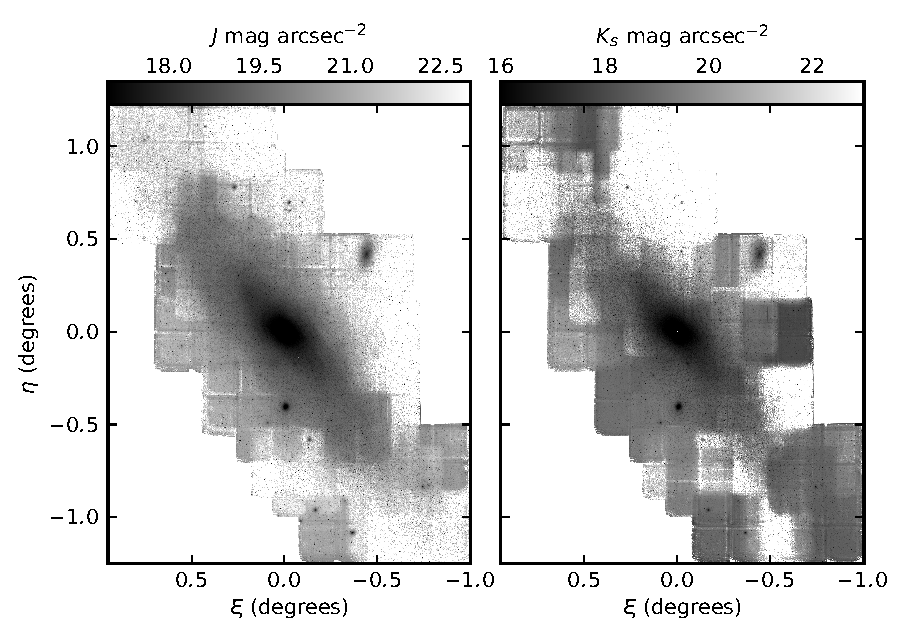
\includegraphics[width=3.5in]{figs/raw_mosaics}
\caption{Median sky subtracted WIRCam $J$ (left) and $K_s$ (right) mosaics of M31.}
\label{fig:raw_mosaics}
% made with skysubpub/mosaic_plots.py
% + skysubpub/raw_mosaic.py
\end{figure}

Despite our attention thus far to real-time sky flat fielding, and median sky image subtraction, we have not achieved our goal of recovering the true NIR surface brightness of M31.
In \Fig{raw_mosaics} we plot mosaics (assembled using \sw{Swarp}) from \androids\ frames processed thus far with the pipeline discussed in \Sec{reduction}--\Sec{photocal}.
Although these basic image preparations dramatically improve image quality the \iiwione\ pipeline (particularly with regards to flat fielding performance), we see that classical NIR sky subtraction has fundamentally limited accuracy.
Classically, the true value of the sky on the disk of M31 is lost by the temporal and spatial variations of skyglow between disk and sky field observations.

To advance on our goal, we demonstrate in this section how the residual sky bias in each observation can be inferred from information in the overlaps of pairs of images in the mosaic.
Each classically sky subtracted image of the M31 disk is a combination of the true surface intensity, $I_i$, and a residual sky intensity, $\epsilon_i$.
Consider a pair of images, $i$ and $j$, that overlap on the galaxy: their difference is $(I_i+\epsilon_i) - (I_j+\epsilon_j) = \epsilon_i - \epsilon_j$.
Given this measurement $\epsilon_i - \epsilon_j$ of residual sky intensity, we introduce \emph{sky offsets}, $\Delta$, for each observation so that

\begin{equation}
    (I_i + \epsilon_i - \Delta_i) - (I_j + \epsilon_j - \Delta_i) \rightarrow 0,
\end{equation}

\noindent and the intrinsic intensities cancel, $I_i - I_j = 0$.
Given a single pair of images, the inference of $\Delta_i$ and $\Delta_j$ is degenerate given the single difference image, $\epsilon_i-\epsilon_j$.
But in a mosaic, each image is coupled (has overlapping domain) with many other images, and the mosaic itself can be considered as a network of coupled images.
If we model the residual sky intensity $\epsilon_i$ as having a simple shape across the observed images, the single offset $\Delta_i$ will minimize all difference images involving image $i$.
That is, sky offsets can be chosen by the optimization of

\begin{equation}
    \sum_{\forall i,j} [(\epsilon_i - \epsilon_j) - \Delta_i + \Delta_j] \rightarrow 0
    \label{eq:scalartheoryobj}
\end{equation}

\noindent over all coupled image pairs $(i,j)$ in the mosaic.
Note that absolute uniqueness is not guaranteed.
In the limit that sky offsets $\Delta_i$ are drawn from a Gaussian distribution, with standard deviation $\sigma_\Delta$, the absolute brightness of the whole mosaic will be uncertain by $\sigma_\Delta / \sqrt{N_\mathrm{images}}$.
The consequences of this uncertainty are revisited in \S\todo{TODO}.

\subsection{Implementations}
\label{sec:offset_algos}

The sky offset optimization summarized in \Eq{scalartheoryobj} is difficult to implement because it is over-constrained, requiring a non-linear optimization.
Any single image is connected in a network (visualized in Fig. \todo{todo}) with others; and any error in the surface brightness \emph{shapes} of fields will result in an imperfect match.
In this work, we consider two implementations of \Eq{scalartheoryobj}.
First, we review the \sw{Montage} software package in \Sec{montage_algo}, and then introduce an alternative in \Sec{msrnm_algo}.

\subsubsection{Montage}
\label{sec:montage_algo}

\sw{Montage} is a FITS mosaicing package \citep{Berriman:2008} originally written for the 2MASS survey, and includes sky offset estimation (background rectification, in their terminology) functionality.
In that software, images are rectified onto a mosaic pixel grid, and difference images are computed among overlapping images.
Sky offsets are then chosen iteratively by looping through each image pair and choosing the offset needed to minimize the difference image of that pair, counting previous sky offset estimates.
That is, at each step the sky levels of the two images are increased and decreased by half the total intensity difference.
Sky offsets are refined over several loops through the entire set of overlapping image pairs until convergence is reached (adjustments to sky offsets diminish below a threshold).
Although this iterative implementation of sky offset optimization is elegant, its accuracy has never been formally analyzed in literature.
In particular, we are interested in the robustness of Montage sky offsets against local minima in the $N$-dimensional solution space of sky offsets, given a mosaic of $N$ independent images.

\subsubsection{A New Implementation based on the Multi-Start Reconverging Downhill Simplex}
\label{sec:msrnm_algo}

As an alternative to the iterative algorithm used by \sw{Montage}, we introduce here an implementation based on the \cite{Nelder:1965} Downhill-Simplex algorithm.
Like \sw{Montage}, our pipeline begins with a set of images resampled to a common pixel grid in an Aitoff projection with the native WIRCam pixel scale (0.3 \arcsec/pixel).
For this we use \sw{Swarp} \citep{Bertin:2002} in resample-only mode.
We identify overlaps between images in a brute-force fashion according to their frames in the mosaic pixel space, defined by the \texttt{CRPIX} and \texttt{NAXIS}$i$ header values of the resampled images.

For each overlapping image pair, we compute a difference image, and ultimately a median difference, $\langle \vect{I}_i - \vect{I}_j \rangle$.
While computing the median difference, we mask bad pixels using weight maps (propagated by \sw{Swarp}) and expand this mask with sigma clipping.
Along with a difference estimate, we also record the area $A_{ij}$ of unmasked pixels in the overlap, and the standard deviation of the difference, $\sigma_{ij}$.

Let us define the objective function that encapsulates the effect of scalar sky offsets on reducing the intensity difference between coupled images:

\begin{equation}
    \mathcal{F} \left(\Delta_1,\ldots,\Delta_n \right) = \sum_{i,j} \mathcal{W}_{ij} \left( \langle \vect{I}_i - \vect{I}_j \rangle - \Delta_i + \Delta_j \right)^2,
    \label{eq:objf}
\end{equation}

\noindent which we intend to minimize by finding the optimal set of scalar sky offsets $\Delta_i$ for each of the detector fields $i$.
Note that each coupled image pair is its own term in the objective summation, and that there are as many degrees of freedom ($\Delta_i$) as there are images in the mosaic.
Each coupling is tempered by a weighting term $\mathcal{W}_{ij}$:

\begin{equation}
    \mathcal{W}_{ij} = \frac{A_{ij}}{\sigma_{ij}},
\end{equation}

\noindent so that more priority is given to couplings of larger areas ($A_{ij}$), and small standard deviations of their difference images ($\sigma_{ij}$).

Note that the objective function in \Eq{objf} puts no constraint on the net sky offset: $\sum \Delta_i$.
Assuming that sky subtraction errors are normally distributed, and not biased, sky subtraction offsets should not add a net amount of flux to the mosaic.
Fortunately, it is possible to impose this constraint \textit{post facto} by subtracting the mean offset from the sky offsets:

\begin{equation}
    \Delta_i^* = \Delta_i - n^{-1}\sum_{j=1}^n \Delta_j.
    \label{eq:netzero}
\end{equation}

Given the image coupling records, we optimize the set of $\Delta_i$ using the \cite{Nelder:1965} (NM) downhill simplex algorithm.
This NM algorithm has the advantage of being naturally multi-dimensional, and being able to work without knowledge of the gradient of the objective function.
Instead, the NM algorithm operates by constructing a geometric simplex of $N+1$ dimensions that samples the sky offset parameter space.
By evaluating the objective function at each vertex of the simplex, the NM algorithm adapts simplex's shape to ultimately contract upon a minimum.

But NM has two weaknesses.
First, it is a \emph{greedy} optimizer that will converge into any local minimum, without necessarily seeking the global minimum.
Second, for high-dimension optimizations (many fields in the mosaic), the NM may fail to converge in a reasonable number of objective function evaluations \citep{Neumann:2006}.
Without solving these issues, a minimization of \Eq{objf} with an off-the-shelf NM code yields a mosaic with obvious discontinuities across fields.
To solve the first problem, we develop a Multi-Start Reconverging NM (MSRNM) downhill simplex driver.
This algorithm allows the NM to cumulatively cover a larger portion of parameter space to probabilistically ensure convergence into a global optimum.

Several approaches have been made in the literature to globalize the NM algorithm in the high-dimensional case.
\cite{Harris:2001} use the NM simplex to fit stellar populations, of roughly 50 parameters, to colour magnitude diagrams in their \sw{StarFISH} application.
Solving for scalar sky offsets in this WIRCam survey has roughly the same degree of complexity.
In the case of \sw{StarFISH}, \citeauthor{Harris:2001} combine the NM simplex optimization with brute force line searches.

An initial grid search indicates a rough starting point for the simplex.
The simplex is allowed to converge upon as minimum through the standard NM algorithm.
Retaining the best point, the other points in the simplex are inflated, and the simplex is again allowed to converge upon a minimum---hopefully the original.
Yet this minimum may still be a local minimum.
To guard against this, points near the minimum are probed.
If the point is more ideal, then that direction of parameter space is searched until the objective function begins to increase.
This random linear search through parameter space is repeated several thousand times.

Another globalization recipe is to start the simplex from a large ensemble of starting positions in parameter space. The global minimum of the objective function should be accessible to the NM algorithm from some portion of the imaginable starting parameter space. An advantage of this is that each start of the downhill simplex can be carried out in parallel on a computing cluster. There are recipes in the literature for choosing the best ensemble of starting simplexes: some based upon a running memory of past downhill simplex runs, and others simply based upon having a uniform coverage of parameter space \citep[\eg][]{Luersen:2004,Wolff:2004}.

The globalization strategy developed here is borrows from the techniques in the literature.
\todo{(add citations.)}
While it is not proven ideal, or most efficient, algorithm, this strategy is easy to implement and provides adequate results.
This strategy wraps the core NM algorithm with multiple random starting positions, and multiple restarts at each converged location until a stable---and global---minimum is found.
Hence this technique is informally termed the Multi-start Reconverging Nelder Mead Simplex (MSRNM).

\paragraph{Multi-start} First, a total of $N_s$ starts of the NM algorithm are designated.
We find that $N_s=1000$ is quite sufficient for an optimization with 39 parameters (such as the fitting of $\Delta_B$ block offsets in mosaic, see \Sec{hierarchical_algo}).
For each start, an initial simplex is generated randomly.
Since each point in the $N$ by $N+1$ simplex is a suggested sky offset for a given field, each offset is randomly sampled from the expected distribution of image-to-image sky offsets.
That is, a normal distribution of mean zero intensity, and standard deviation of $\sigma_\mathrm{start}$.
To ensure that the parameter space is well covered, we design $\sigma_\mathrm{start}$ to be $10\times$ greater than the dispersion of image-to-image differences.

Each initial simplex is allowed to converge according to the NM algorithm.
A simplex is deemed converged once each point has changed by no more than $10^{-4}$ of the previous iteration, or the objective function's value has changed by no more than $10^{-4}$ of the previous iteration. 

\paragraph{Restart} Upon convergence, the optimal point in the simplex, $\vect{p}$, is recorded.
A new simplex is then generated where one vertex is $\vect{p}$, and the rest are $\vect{p}+\vect{\delta}$ where $\vect{\delta}$ is a normal random variable of mean zero, and standard deviation $\sigma_\mathrm{restart}$.
That is, the simplex of the restart retains one vertex upon the previously found minimum, while the other vertices surround that minimum.
If the minimum is indeed the global minimum, then the NM algorithm will quickly reconverge.
But more often than not, the other random vertices will probe an even better parameter space, causing the NM restart to converge upon a new minimum.
When a new minimum is found, the process of restarting is repeated until the same minimum is consecutively arrived upon.
Like $\sigma_\mathrm{start}$, there is flexibility in choosing $\sigma_\mathrm{restart}$; generally $\sigma_\mathrm{start}$ should be on the order of the observed image-to-image difference dispersion, not not necessarily as large as $\sigma_\mathrm{start}$.
\todo{Cite numerical recipes for this algorithm design? Or it is from elsewhere?}

\subsection{Hierarchical sky offset optimization}
\label{sec:hierarchical_algo}

Sky offset optimization is challenging because of dimensionality. Assuming that sky residuals are \emph{constant} across a frame, each image frame represents a new dimension ($\Delta_i$) in the optimization. Considering that the WIRCam array produces four image frames for every exposure, the combined 2007B and 2009B data sets consist of 3924 $J$ and 4972 $K_s$ image frames that cover the disk of M31. Such a large optimization is computationally ambitious, but also needless.

Our sky optimization algorithm breaks the optimization of sky offsets into three sequential steps, which we call \emph{hierarchical sky offset optimization}.

The 2007B and 2009B WIRCam surveys observed a total of 39 \emph{fields} across the M31 disk (illustrated in \Fig{fieldmap}).
Each WIRCam field is imaged with four detectors, arranged in a $2\times 2$ grid.
Let us define a \emph{detector field} as the collection of images that are taken with a given detector, at a given field.
Images in a detector field have the greatly simplifying property of all overlapping across a dominant section of the image frame.

Thus our M31 WIRCam mosaics are assembled in three steps.
In Step 1 we combine the frames in a detector field to produce a \emph{detector field stack}.
The combined 2007B and 2009B surveys have 156 such stacks per filter.
In Step 2, the four detector field stacks within each field can be fitted into a \emph{block}.
A block is a fundamental unit of the mosaic, as all images that are combined within a block were observed under contemporaneous sky conditions.
Finally, in Step 3, the 39 blocks can be fitted into a galaxy-wide mosaic for each filter.

Note that detector field stacks can be made with a simple median-combination of frames in a detector field.
Since the frames are dithered, the periphery of the detector field is covered by subsets of the frames.
A simple median combination, then, produces edges that have background levels that are biased compared to the central pixels that are covered by the entire frame set.
A solution is to estimate offsets for each frame compared to this first detector field stack.
Offsets are computed as the median of the difference image between the stack and individual image frames.
The original image frames, now with offsets applied, are re-combined into a detector field stack image.
Now edge-effects are smaller.
Nonetheless, offsets are estimated a second time to produce a finalized detector field stack image.
Let us denote the offsets applied to individual frames at this first stage as $\Delta_F$.

In the second hierarchical level, we combine sets of four detector field stacks into blocks.
Here we must use the non-linear optimization algorithms detailed in \Sec{montage_algo} or \Sec{msrnm_algo}.
Let us denote the offsets of stacks into blocks as $\Delta_S$. Finally, we again use our offset optimization algorithms to combine blocks into a mosaic. The sky offsets applied to blocks at this stage are labelled $\Delta_B$. We also measure a net offset: $\Delta_\Sigma = \Delta_F + \Delta_S + \Delta_B$ for each frame.


\section{Analysis of Scalar Sky Offsets}
\label{sec:scalaranalysis}

We can now present the fruits of our WIRCam pipeline and sky offset optimization with \Fig{scalar_mosaics}.
Compared to our mosaics without sky offsets, \Fig{raw_mosaics}, it is clear that sky offset optimization is essential for assembling wide-field NIR mosaics.
Note that these mosaics are not yet perfect; field-to-field discontinuities remain, and large-scale sky residuals perturb the outer M31 disk.

\begin{figure}[t]
	\centering
		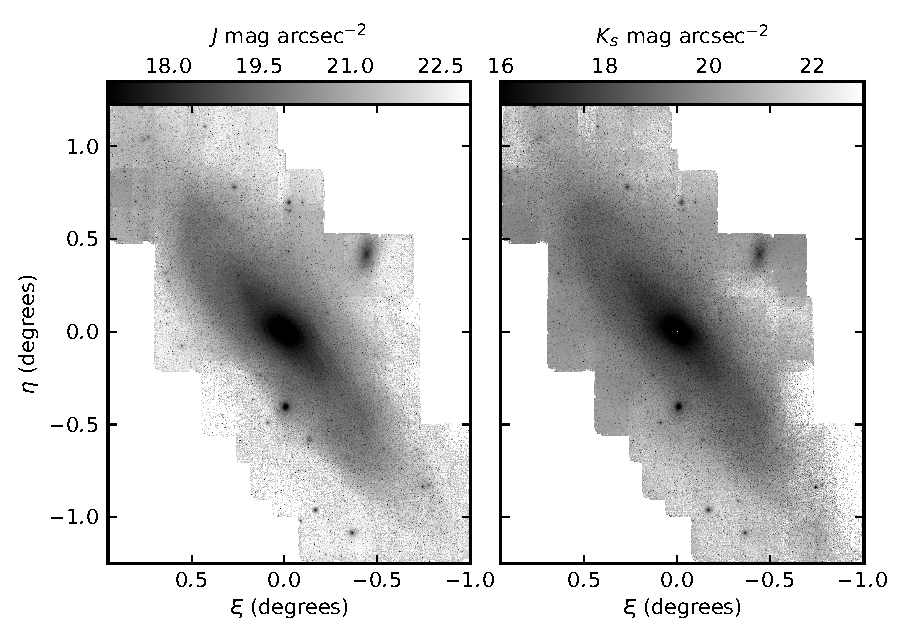
\includegraphics[width=3.5in]{figs/scalar_mosaics}
	\caption{Scalar-sky fitted WIRCam $J$ (left) and $K_s$ (right) mosaics of M31. Note the qualitative improvement compared to the original, median sky-subtracted, images in \Fig{raw_mosaics}.}
	\label{fig:scalar_mosaics}
	% made with skysubpub/mosaic_plots.py
\end{figure}

\subsection{Amplitudes of Sky Offsets}
\label{sec:offset_amplitudes}

The distribution of scalar sky offsets provide an excellent characterization of sky subtraction uncertainties when using sky-target nodding.
Recall that sky offsets are optimized hierarchically: WIRCam frames are fitted to stacks, stacks are fitted into blocks of four contemporaneously-observed WIRCam detector fields, and these blocks are fitted into a mosaic.
\Tab{offset_hierarchy} lists the standard deviations of these offset distributions with respect to the typical sky level observed in the $J$ and $K_s$ bands.

% NOTE ON MEAN SKY LEVELS
% According to andpipe/wircam/calibset/mosaic/scalar_offset_hierarchy.py:
% Mean J Level: 894.19 muJy. Mean Ks Level: 19902.80 muJy
% But note that in WIRCam instrumental ADU/s, teh mean sky levels are:
% J: 122 ADU/s, Ks: 488 ADU/s. see $andpipe/wircam/skyanalysis/mean_sky_level.py

Note that the sky offsets, as a percentage of sky level, are comparable in the $J$ and $K_s$ bands, despite the sky glow being $\sim 4\times$ brighter in $K_s$ than $J$ (see \Fig{net_sky_level}).
This indicates that spatiotemporal variations in the NIR sky are monochromatic.

Within the hierarchy of sky fitting, simply fitting frames to a stack (with $\Delta_F$) is most significant: a correction on the order of 2\% of the sky intensity.
Fitting these blocks into a mosaic ($\Delta_B$) is a further $\sim 1$\% correction.
The offsets to fit a stack into a block ($\Delta_S$) of four detector field stacks are smallest: 0.1\% of the sky level.
This suggests that on the scale of the $2\times 2$ WIRCam array, the contemporaneously observed detector frames are subjected to nearly identical biases in sky background.
But overall, the temporal and spatial lags of sky-target nodding induce a 2\% uncertainty in the sky level at the target.
It is this level of uncertainty that sky offset optimization that must be diminished to transform uncorrected mosaics (\Fig{raw_mosaics}) to ones that show the disk with fidelity (\Fig{scalar_mosaics}).

A comparison between the net sky offsets applied to the 2007B and 2009B data sets is provocative.
Although the 2009B dataset employed rapid sky-target nodding to minimize temporal lags between disk and sky sampling, the magnitude of sky offsets in the 2007B and 2009B semesters is comparable.
This implies a limit to the absolute sky level accuracy that can be expected: the minimal 40~sec lag between sky and target samples, combined with a 1--$2\arcdeg$ nod across the sky, allows the sky level to change by 2\%.
Reducing this latency, and this nodding distance, is impossible in WIRCam observations of M31.
Thus by the metric of \Tab{offset_hierarchy}, the expensive 2009B observing approach does not return full dividends.


\begin{table}[t]
\centering
\caption[Hierarchy of scalar sky offsets]{Hierarchy of scalar sky offsets (using \texttt{FW100K} RT flat fielding, and median sky subtraction).
The `Total' sky offsets track the net offset of individual WIRCam image frames into the fitted mosaic.
$\langle I_\mathrm{sky}\rangle$ is taken as the instantaneous sky level for the images being sampled (see \Fig{net_sky_level} for the distribution of levels).
Offset distributions are also presented in units of the instrumental count rate, ADU $s^{-1}$, of CFHT/WIRCam.}
\label{tab:offset_hierarchy}
% made with $andpipe/wircam/calibset/mosaic/scalar_offset_hierarchy.py
\begin{tabular}{ll|rr|rr}
% \hline
&  & \multicolumn{2}{c|}{$J$} & \multicolumn{2}{c}{$K_s$} \\ % \cline{3-4} \cline{5-6}
% \hline
Offset Type & Sem. & $\sigma_\Delta$ & $\frac{\sigma_\Delta}{\langle I_\mathrm{sky}\rangle }$ & $\sigma_\Delta$ & $\frac{\sigma_\Delta}{\langle I_\mathrm{sky}\rangle }$ \\
& & \tiny{($\mu$Jy arcsec$^{-2}$)} &  \tiny{(\%)} & \tiny{($\mu$Jy arcsec$^{-2}$)} &  \tiny{(\%)} \\
\hline
\multirow{2}{*}{$\Delta_F$} & 07B & 18.5 & 2.37 & 39.7 & 1.79 \\
% \hline
& 09B  & 15.2 & 1.70 & 39.5 & 2.26 \\
\hline
\multirow{2}{*}{$\Delta_S$} & 07B & 1.1 & 0.14 & 1.9 & 0.09 \\
% \hline
& 09B & 1.1 & 0.11 & 1.5 & 0.08 \\
\hline
\multirow{2}{*}{$\Delta_B$} & 07B & 9.8 & 1.27 & 19.2 & 0.91 \\
% \hline
& 09B &  7.0 & 0.73 & 26.6 & 1.43 \\
% \hline
\hline
\multirow{2}{*}{$\Delta_\Sigma$} & 07B &  20.4 & 2.61 & 43.4 & 1.99 \\
% \hline
& 09B &  16.3 & 1.81 & 38.0 & 2.15 \\
% \hline
\end{tabular}
\end{table}

\subsection{Acceptability of Sky Offsets}
\label{sec:offset_acceptability}

Recall that scalar sky offsets were initially introduced as nudges in intensity to overcome uncertainty in the sky level of detector field stacks.
For sky offsets to be considered acceptable, we demand that the offsets applied to blocks, $\Delta_B$ be consistent with the sky level uncertainty of the blocks themselves.
We can conservatively measure the sky uncertainty as the dispersion of $\Delta_F$ frame offsets in a stack: $\sigma_{\Delta_F}$.
Thus if sky offsets fitted between blocks are statistically permissible, then $\Delta_B \lesssim \sigma_{\Delta_F}$.
In \Fig{offset_ratio_map}, we plot a field map (in the same spatial configuration as \Fig{fieldmap}) painted with the values of $\Delta_B / \sigma_{\Delta_F}$ for each detector field in the $J$ and $K_s$ mosaics.
The sky offsets are indeed distributed within the uncertainty budgeted by $\sigma_{\Delta_F}$: the sky offsets are statistically acceptable.

\begin{figure}[t]
\centering
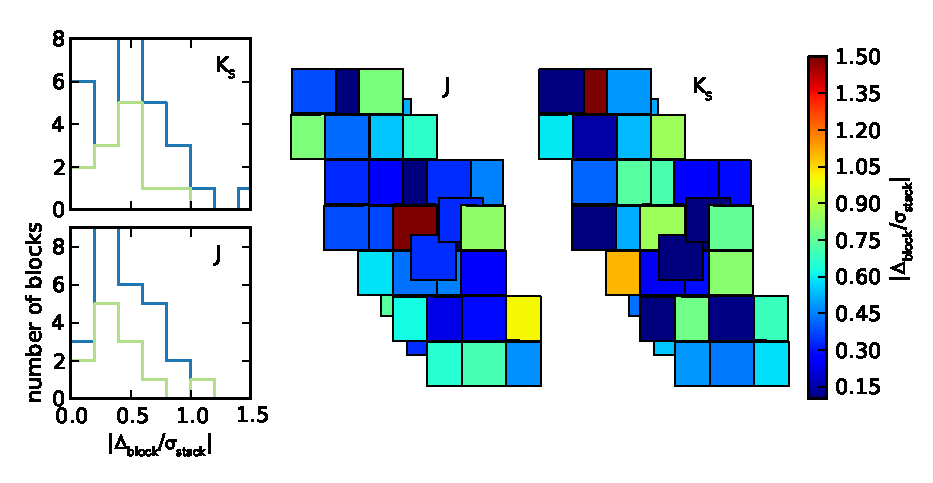
\includegraphics[width=\columnwidth]{figs/offset_ratio_map_enhanced}
\caption{Acceptability of $J$ and $K_s$ scalar sky offsets between blocks, as measured by the ratio of $\Delta_B/\sigma_{\Delta_F}$.}
\label{fig:offset_ratio_map}
% made with skyoffset/offsetratiomap.py
% TODO need to fix colour scheme of the histograms
\end{figure}

Another demonstration of the veracity of these sky offsets is given in Fig. \todo{TODO}, where we plot a timeseries of both directly measured sky levels, and sky levels interpolated on disk observations via sky offsets.
Note how remarkably continuous the sky level is from sky to disk observation; compared to the sky level timeseries of stationary sky fields, the variations in the sky level interpolated on the disk appear real.
Through the sky target nodding and sky offset optimization, we \emph{have} effectively measured the level of the sky on M31.
The variability of the sky in these timeseries will be further pursued in \S \todo{TODO}.

\subsection{Residual Image Level Differences}
\label{sec:residual_diffs}

Although the scalar sky offsets are statistically valid, they are not perfect prescriptions against the sky subtraction uncertainties of each image stack---that much is visually true.
A measure of the limitation of sky offset fitting are the residual image level differences between coupled blocks, $(\vect{I}_i - \Delta_{B,i}) - (\vect{I}_j - \Delta_{B,j})$, after the sky offsets $\Delta_{B,i}$ have been optimally fitted to each block.

\Tab{fw100k_medsky_scalar_resid_diffs} lists distributions of both image level differences between coupled blocks, before and after the application of scalar sky offsets.
Uncorrected, the ensemble of coupled blocks have a mean intensity difference of $\sim 1\%$ of the typical sky background intensity.
Scalar sky offsets decrease the differences between overlapping fields to $\sim 0.2\%$.

With \Fig{fw100k_medsky_scalar_resid_sbfrac} we can visualize these block-to-block residual differences as a fraction of the local surface brightness.
Note that throughout the bright inner disk of M31, block-to-block residuals are negligible compared to the disk signal; but at the mosaic periphery ($R\sim 20$~kpc), the field-to-field residuals become comparable to, or greater than, the disk surface brightness.
The poor fit is driven primarily by diminishing disk signal, rather than poor convergence of sky offsets.
This can be seen by plotting the magnitude of block-to-block residuals (in units of sky brightness) in \Fig{fw100k_medsky_scalar_resid_skyfrac}.
There, significant residuals are distributed throughout the disk, rather than the low-SB periphery of the mosaic.
\comment{Note that these residuals can be as much as 2\% of the sky brightness! This is bad; used to be 0.02\%! What happened?}

Of course, it is precisely this residual image level difference that was sought to be minimized as part of the optimization's objective function (\Eq{objf}).
The inability of scalar sky offset optimization to eliminate residual image differences should not be interpreted as a failure to detect the global minimum; the MSRNM optimization algorithm appears robust in arriving at this offset solution set.
Evidence of this can be seen in \Fig{fw100k_medsky_scalar_resid_sigmafrac}, where block-to-block network connections are coloured by the ratio of the residual block-to-block intensity difference to the uncertainty in the block-to-block difference image.
The sky offsets solved by the MSRNM algorithm are within the uncertainties of the difference images themselves; better scalar sky offsets \emph{cannot} be made with the WIRCam blocks our pipeline has produced.
Nonetheless, block-to-block surface brightness discontinuities are plainly seen in \Fig{scalar_mosaics}.

An interpretation of this failure is that sky background residuals are not entirely scalar across WIRCam blocks.
Our discussion in \Sec{skyflatstability}, and particularly \Fig{frame_residuals_M31-37_Ks_fw100k_medsky}, indicate that flat field variability, and sky background variability can affect the shape of WIRCam fields.

\begin{table}[t]
\centering
\caption[Coupled block differences and residual differences after
scalar sky offsets]{Coupled block intensity differences and residual intensity differences after application of scalar sky offsets: 25th, 50th and 75th percentiles of distribution.
Differences are presented as a percent of the mean sky level seen by observations in each band.
}
\begin{tabular}{lccc}
& \multicolumn{3}{c}{Coupled Block
$\langle I_i - I_j\rangle / \langle I_\mathrm{sky} \rangle$ (\%)} \\
& 25th & 50th & 75th \\
\hline
$J$, uncorrected & 0.47 & 0.91 & 1.70 \\
$J$, scalar offset & 0.05 & 0.09 & 0.18 \\
\hline
$K_s$, uncorrected & 0.42 & 0.90 & 1.43 \\
$K_s$, scalar offset & 0.02 & 0.05 & 0.08 \\
\hline
\end{tabular}
\label{tab:fw100k_medsky_scalar_resid_diffs}
% $andpipe/wircam/calibset/mosaic/residuals_table.py
\end{table}

\begin{figure}[t]
\centering
\includegraphics[width=3.5in]{figs/fw100k_medsky/networks/scalar_resid_sbfrac}
\caption{Map of residual block-to-block surface brightness differences as a fraction of mean local surface brightness, after scalar fitting.
  This graph mimics the spatial distribution of the 2007B and 2009B WIRCam fields (\Fig{fieldmap}), but the field boxes have been exploded to allow room for lines to connect coupled blocks.
}
\label{fig:fw100k_medsky_scalar_resid_sbfrac}
% made with $andpipe/wircam/calibset/mosaic/networkmap.py
\end{figure}

\begin{figure}[t]
\centering
\includegraphics[width=3.5in]{figs/fw100k_medsky/networks/scalar_resid_skyfrac}
\caption{Map of residual block-to-block surface brightness differences as a fraction of the mean sky level, after scalar fitting.}
\label{fig:fw100k_medsky_scalar_resid_skyfrac}
% made with $andpipe/wircam/calibset/mosaic/networkmap.py
\end{figure}

\begin{figure}[t]
\centering
\includegraphics[width=3.5in]{figs/fw100k_medsky/networks/scalar_resid_sigmafrac}
\caption{Map of residual block-to-block surface brightness differences as a fraction of the standard deviation of the difference image, after scalar fitting.}
\label{fig:fw100k_medsky_scalar_resid_sigmafrac}
% made with $andpipe/wircam/calibset/mosaic/networkmap.py
\end{figure}


\subsection{Usefulness of Planar Sky Offsets}

\label{sec:planar_offset_analysis}

\todo{\begin{enumerate}
    \item mosaic plot of montage planar offsets
    \item table or histogram with distribution of planar slopes in units of mag per arcsec? or percent of sky per arcsec?
    \item residual network plot showing block-to-block residuals in percent of sky. Compare to \Fig{scalar_relresidnet}.
\end{enumerate}
}



\section{Systematic Uncertainties in Surface Brightness Reconstruction}
\label{sec:systematics}

\begin{figure}[t]
    \centering
        \includegraphics[width=3.5in]{figs/sbdiff/scalar_irac36_sbdiff.pdf}
    \caption{Maps of $J-[3.6]$ and $K_s-[3.6]$ surface colour inferred from the scalar-sky fitted WIRCam mosaics (see \S\ref{sec:scalar}--\ref{sec:scalaranalysis}) and Spitzer/IRAC 3.6~$\mu$m image \citep{Barmby:2006}. Note that the IRAC map crops the \androids/WIRCam footprint.}
    \label{fig:scalar_irac36_sbdiff}
    % make with skysubpub/diffplots.py
\end{figure}

\begin{figure}[t]
    \centering
        \includegraphics[width=3.5in]{figs/sbdiff/altplanar_irac36_sbdiff.pdf}
    \caption{Maps of $J-[3.6]$ and $K_s-[3.6]$ surface colour inferred from the planar-sky fitted WIRCam mosaics (see \S\ref{sec:scalar}--\ref{sec:scalaranalysis}) and Spitzer/IRAC 3.6~$\mu$m image \citep{Barmby:2006}. Note that the IRAC map crops the \androids/WIRCam footprint.}
    \label{fig:altplanar_irac36_sbdiff}
\end{figure}

Sky offsets produce a mosaic that is rigorously optimal only in the sense of field-to-field surface brightness continuity---not absolute sky subtraction. In this section, we attempt to gauge the systematic surface brightness error inherent in the sky offset technique.

\subsection{Comparison to Spitzer/IRAC Images}

Systematic uncertainties can be explored by comparing our WIRCam mosaics to well-calibrated images of M31, and looking for colour discrepancies.
A template for the old stellar disk, is the 3.6~$\mu$m Spitzer/IRAC map, presented in \cite{Barmby:2006}, which avoids sky subtraction uncertainties inherent in ground-based observation.
In \Fig{scalar_irac36_sbdiff} we compare the scalar-fitted mosaics against the 3.6~$\mu$m image. Generally the $J-[3.6]$ and $K_s-[3.6]$ colors decrease with disk radius, but increase in the star-forming regions because of hot dust emission. Both the scalar-fitted $J$ and $K_s$ mosaics are reddened in the south-eastern corner, which we interpret as a systematic \emph{over-subtraction} of the WIRCam NIR sky. In $J-[3.6]$ and $K_s-[3.6]$ maps realized with planar-fitted sky, \Fig{altplanar_irac36_sbdiff}, a similar, though stronger, systematic sky error is seen. This result qualitatively illustrates the greater potential for systematic sky errors when planar sky correction freedom is permitted across the $20\times 20$ arcmin WIRCam blocks.

\subsection{Comparison to \sw{Montage}-fitted images}

\begin{figure}[t]
    \centering
        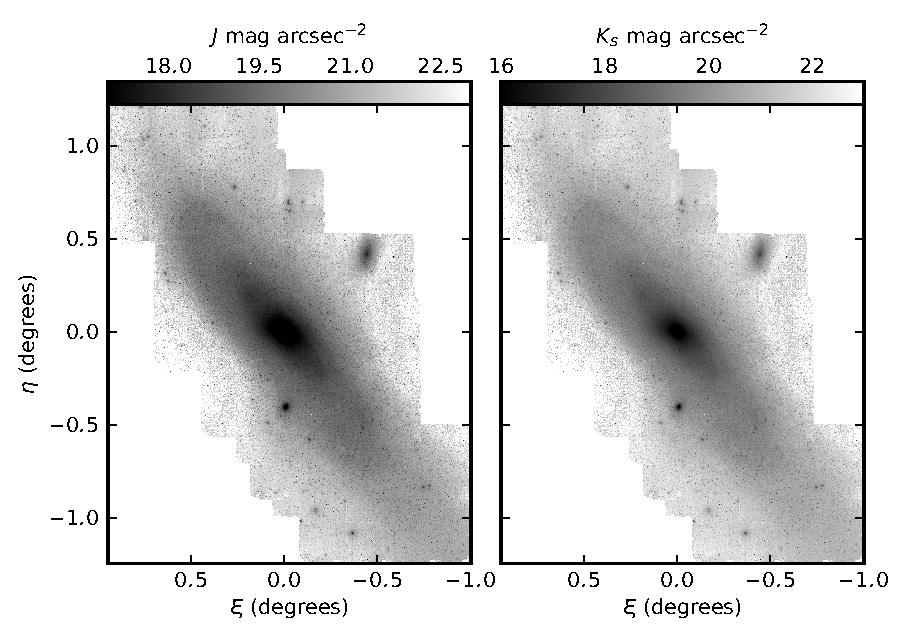
\includegraphics[width=3.5in]{figs/montage_planar_mosaics.pdf}
    \caption{Montage-generated $J$ and $K_s$ maps. Compare to the equivalent simplex maps, Figs.~\ref{fig:scalar_mosaics}~and~\ref{fig:planar_mosaics}. Pixels with negative surface intensity, after sky offset correction, are masked with white.}
    \label{fig:montage_planar_mosaics}
    % make with skysubpub/mosaic_plots.py and skyoffset/montageoffsets.py
\end{figure}

\begin{figure}[t]
    \centering
        \includegraphics[width=3.5in]{figs/sbdiff/montage_irac36_sbdiff.pdf}
    \caption{Maps of $J-[3.6]$ and $K_s-[3.6]$ surface colour inferred from the \sw{Montage}-fitted WIRCam mosaics (see \Fig{montage_planar_mosaics}).}
    \label{fig:montage_irac36_sbdiff}
    % make with skysubpub/diffplots.py
\end{figure}

\begin{figure}[t]
    \centering
        \includegraphics[width=3.5in]{figs/sbdiff/altplanar_jk_sbdiff.pdf}
    \caption{$J-K_s$ colour maps realized by the simplex planar sky fitting algorithm (left) and \sw{Montage} (right).}
    \label{fig:altplanar_jk_sbdiff}
    % make with skysubpub/diffplots.py
\end{figure}


Although this paper advocates a sky offset optimization based on the \cite{Nelder:1965} Downhill Simplex algorithm, other tools exist for solving sky background corrections.
A popular package is \sw{Montage} \citep{Berriman:2008}.
Like the algorithms presented in this paper, \sw{Montage} uses the network of image-to-image differences to infer sky offsets.
Rather than simultaneously solve for all offsets, \sw{Montage} uses an iterative algorithm: offsets are proposed that arithmetically solve one pair of images, and that offset change is propagated into the adjacent pair, which are again arithmetically offset, and so forth.

Figure~\ref{fig:montage_planar_mosaics} shows mosaics generated by \sw{Montage}, allowing for planar sky offsets.
These surface brightness realizations lead to $J-[3.6]$ and $K_s-[3.6]$ maps in \Fig{montage_irac36_sbdiff}.
Comparing the simplex-optimized color map (\Fig{altplanar_irac36_sbdiff}) against the \sw{Montage} realization, it is plain that the two algorithms find different sets of globally optimum sky offsets.
And neither of the solutions is optimal in the sense of absolute calibration.

Another useful comparison is \Fig{altplanar_jk_sbdiff}, where $J-K_s$ color maps are realized by both the simplex planar-fitting and \sw{Montage} algorithms.
Unlike the comparisons against $[3.6]$, these color maps test the entire \androids\ footprint.
Absolute calibration of the NIR surface brightness is a clear requisite before these images are scientifically useful beyond the inner disk.

\subsection{Monte Carlo Analysis of Systematic Surface Brightness Uncertainties}

\begin{figure}[t]
\centering
\includegraphics[width=\columnwidth]{figs/bootstrap_sb_rms.pdf}
\caption{Maps of bootstrap RMS surface brightness in $J$ (left) and $K_s$ (right) mosaics.
White contours identify RMS levels of 0.05 (solid), 0.1 (dashed) and 0.2 (dash-dot) mag arcsec$^{-2}$.}
\label{fig:bootstrap_sb_rms}
% made with skyoffset/bootstrap.py BootstrapRMSPlot
\end{figure}

\begin{figure}[t]
\centering
\includegraphics[width=\columnwidth]{figs/bootstrap_recovery_map.pdf}
\caption{Dispersions ($1\sigma$) in the difference of expected and observed sky offsets in Monte Carlo realizations of the $J$ (left) and $K_s$ (right) mosaics.
The 2009B fields are plotted over top of the 2007B fields (see \Fig{fieldmap} for spatial reference).}
\label{fig:bootstrap_recovery_map}
% made with skyoffset/bootstrap.py OffsetRecoveryFieldMap
\end{figure}


The difference images presented in the previous section, and particularly \Fig{altplanar_jk_sbdiff}, illustrate how the surface brightness reconstructions of identical data can vary depending on the optimization algorithm.
Here we pose a slightly different question: how are reconstructions affected by the initial conditions of sky errors? We answer this with a Monte Carlo analysis.

A Monte Carlo (MC) realization is generated by perturbing the surface brightness of the corrected blocks with a sky error drawn (with replacement) from the ensemble of block sky offsets observed in the original mosaic (\Fig{scalar_mosaics}).
Using the scalar-sky fitting procedure, sky offsets  are optimized against the known sky perturbations.
150 such realizations are made to compile an ensemble of mosaics in both bands.

Figure~\ref{fig:bootstrap_sb_rms} shows the RMS deviation of MC mosaic surface brightness against the original scalar-fitted mosaics. Reconstructed surface brightness in the outer disk can vary $\sim 1$ mag arcsec$^{-2}$, consistent with colour biases in the $J-[3.6]$ and $K_s-[3.6]$ maps.

Another view into this effect is \Fig{bootstrap_recovery_map}, where the standard deviations between expected and realized sky MC offsets is plotted.
These maps show that the typical error in realized offset, compared to input sky perturbation, is 0.05\%--0.10\% of the sky intensity.
One hypothesis is that this sky offset recovery error is due to flexure in the mosaic---where blocks on the mosaic periphery are forced to conform to the surface brightness of more central and tightly coupled blocks.
Yet \Fig{bootstrap_recovery_map} does not show a clear outside-in trend.
The $J$ map (\Fig{bootstrap_recovery_map} [left]) does show a slight north-south trend, but more abundant is the precision with with sky perturbations for the 2009B fields were recovered.

Rather than mosaic flexure, a better model for \Fig{bootstrap_recovery_map} is uncertainties in the \textit{post priori} adjustment for zero net offset (\Eq{netzero}).
Since block sky offsets have approximately Gaussian distributions with dispersions given in \Tab{offset_hierarchy}, the uncertainty in the net offset correction is simply $\sigma(\mathrm{block})/\sqrt{n_\mathrm{blocks}}$.
Considering the dispersions among 2007B block offsets, the expected uncertainty of the zero net offset correction is 0.08\% and 0.09\% of the $J$ and $K_s$ sky intensity, respectively.
The dominant source of uncertainty shown in the MC simulations, Figs.~\ref{fig:bootstrap_sb_rms}~and~\ref{fig:bootstrap_recovery_map}, is the use of an arithmetic mean of offsets to set an absolute zeropoint, not flexure or uncertainty in the network of offsets.
This suggests that external zeropoints could be very useful in replacing \Eq{netzero}. Since no absolutely-calibrated NIR photometry of M31's surface brightness exists, we will discuss a method using panchromatic resolved stellar populations in a future work.


\section{Stability of WIRCam Sky Flats, and Role of Median Sky Subtraction}
\label{sec:skyflatstability}

Let us now consider the consequences of the WIRCam reduction pipeline described thus far in \Sec{reduction}--\ref{sec:scalar}.
In particular, we are interested in the consequences of flat field design choices.
Our construction of skyflats permits one significant choice: how broad should the window of sky images be to reliably capture both pixel-to-pixel sensitivity, and the large scale illumination of the WIRCam detector.
The robustness of skyflats is, on one hand, tempered by the flatness of the NIR sky itself.
Wide-field movies of the NIR sky \citep{Adams:1996} show the NIR sky glow to be akin to a moving cloud system.
As such, the NIR sky seen by WIRCam is never flat—yet by definition a flat field must necessarily be built from an intrinsically uniform illumination across the telescope focal plane.
In producing a NIR sky flat, we hypothesize that the mean shape of the NIR sky over a timespan is flat.
By maximizing the time window we can marginalize over as many sky shapes as possible to produce an unbiased skyflat.
This notion is embodied in the \texttt{QRUN} sky flats that combine hundreds of sky shapes captured across several days.
But this also assumes that WIRCam is a \emph{stable} detector over the period of several days.
In this section, we consider the stability of WIRCam flat fields and argue for the optimal window for building WIRCam sky flats that is both responsive to changes in the WIRCam detector, and robust against sky shape biases.

A first test of the accuracy of the different skyflats is their ability to produce an unbiased sky.
In this test, measuring the median sky shape of flattened sky images, the \texttt{QRUN} sky flats readily fail (see \Fig{qrun_median_sky}).
Axis symmetry, and presence of dust donuts imprinted on the sky, indicate that WIRCam is not mechanically stable over a queue run.
Real-time (RT) sky flats, on the other hand, do produce flat median sky images to within a high accuracy.
But since RT sky flats, such as \texttt{FW100K}, median sky images over similar timescales as the median sky images themselves, this test is less useful.
Instead, in \todo{Fig. TODO} we show a typical sky frame flattened by an \texttt{FW100k} sky flat.
Such images are flat at a level of \todo{TODO}\% of the NIR sky.
Of course, the flattness of the sky is by design! We must ask how these RT sky flats evolve, and whether such flats are actually calibrating the WIRCam gain structure and illumination function, and not simply enforcing a flat sky.

\begin{figure}[t]
\centering
\includegraphics[width=\columnwidth]{figs/1129459_1129489_Ks_queuesky_medsky}
\caption{A typical median sky image from images calibrated by \texttt{QRUN} sky flats.
Although the median sky images vary,  the axis symmetry and dust patterns are indicative of flat fielding bias.
As shown, flat-fielding errors impose sky subtraction biases on the order of 1\% of the NIR sky level, which is unacceptable for this M31 survey.}
\label{fig:qrun_median_sky}
\end{figure}

A simple test of WIRCam's flatfield stability is to monitor how the RT skyflats evolve on scales of hours.
In \Fig{fw100k_movie} we show percent difference images between RT sky flats made at intervals of 15, 30, 60 and 90 minutes after an initial RT sky flat.
After just 30 minutes, the shape of the RT skyflats deviate by 0.5\% from the initial flat field shape.
By 60 minutes, the deviation exceeds 1\%.
Evidently, the WIRCam flat field function is stable on timescales less than 30 minutes---much less than a queue run.

Nonetheless, the spatiotemporal evolution takes many forms.
In some cases (\Fig{fw100k_movie}b) the flat field deviations are axis symmetric, while in others there is a distinct East-West deviation (\Fig{fw100k_movie}ac).
We interpret these patterns as instabilities in the WIRCam illumination function on the scales of minutes.
\comment{It will be interesting to see if there is always asymmetry in staring/07B sky flats where the same sky field is consistently used, and circular symmetry in the 09B ST-nodding fields. I'm not sure what this means, but would imply a correlation with telescope movement or spatial sampling of the sky.}

\begin{figure*}[p]
\centering
\includegraphics[width=7in]{figs/fw100k/fw100k_movie}
\caption{Spatio-temporal evolution of \texttt{FW100K} sky flats, shown as percent difference of the flat fields 15, 30, 60 and 90 minutes after the initial sky flat of the night. Sky flat evolution on three nights is shown: (a) 2009B $K_s$ observing block when the telescope `stared' at a sky field, (b) 2009B $K_s$ observing block with regular sky-target nodding, and (c) a 2007B observing block with sky-target nodding.}
\label{fig:fw100k_movie}
\end{figure*}

An alternative interpretation is that these sky flat deviations are instabilities in the WIRCam detector electronics.
The dominant macroscopic electronic feature in WIRCam flat fields are the amplifier bands.
Each WIRCam detector is divided into 32 horizontal bands (64 pixels high) that are each read out into independent amplifiers.
These amplifiers have gains that result in levels that differ by 10\% in flat field images.
But these different gains appear stable: over the course of an observing block, the mean flat field level of each amplifier band evolved by less than 0.1\% relative to other amplifiers (see \Fig{fw100k_globalamp_timeseries_55136_Ks}) over three hours.
Indeed, the amplifier band signature is absent from the RT skyflat difference images (\Fig{fw100k_movie})\footnote{Quite unlike \Fig{domeflatratio} that compared dome flat and QRUN sky flat shapes.}
Sky flat evolution does appear driven by changes in the large scale detector illumination function, not electronic instabilities.

\begin{figure}[t]
\centering
\includegraphics[width=\columnwidth]{figs/fw100k/fw100k_globalamp_timeseries_55136_Ks.pdf}
\caption{Time evolution of the mean flat field level of amplifier bands in the four WIRCam detectors in RT sky flats made over three hours. Amplifier bands colours are mapped to their order on the array: red lines at the bottom, green in the middle, and red at the top. Although the levels of individual amplifiers differ by 10\%, their order is consistent, indicating that amplifier gain is extremely stable. The jitter is due to chip-to-chip zeropoint normalization (\Sec{flatbuilding}) uncertainty, or measurement biases.}
\label{fig:fw100k_globalamp_timeseries_55136_Ks}
% wircam/skyflat/plots/amp_level_global.py
\end{figure}

Although the WIRCam illumination function appears to vary rapidly, and strongly, we do not see extremely strong sky residuals (\ie \Fig{qrun_median_sky}) in the \texttt{QRUN}-calibrated mosaic (ultimately presented in \todo{\S TODO}).
This can be attributed to the functionality of median sky subtraction (\Sec{mediansky}).
Suppose the disk has a flux of $N$ counts, while the sky brightness is $S$ counts, before flat fielding.
Suppose that both the disk and the paired median sky subtraction image are calibrated with the same flat field, $\mathcal{F}$.
Then the flat fielded, and median sky subtracted, disk image will be $(N + S)/\mathcal{F} - S \mathcal{F}$.
Suppose the same disk image is calibrated with a flat fielded with a sky flat that is biased by a factor $\epsilon$, so that in this case the incorrectly calibrated disk image is $(N + S) / \epsilon \mathcal{F} - S / \epsilon \mathcal{F}$.
The magnitude difference between the correct and incorrect disk surface brightnesses will only be $2.5 \log_{10} \epsilon$.
That is, a 1\% error in the flat field will only perturb the observed disk surface brightness by 0.01~mag.
So long as the disk and sky are observed with the same flat field function, median sky subtraction will nonetheless subtract, and effectively flatten, the sky background of the disk image.

Although the median sky subtraction is effective at flattening the sky background shape induced by bias flat fields, we can nonetheless detect how incorrect flat fielding changes disk surface brightness.
Any time-varying flat-field function that is inadequately measured should be revealed as a distribution of surface brightness estimates on the bright bulge of M31, where flat fielding is more important than sky subtraction accuracy.
In Figures~\ref{fig:frame_residuals_M31-37_Ks_fw100k_medsky} and~\ref{fig:frame_residuals_M31-37_Ks_QRUN} we see the residual shapes of individual WIRCam frames against the median shape of the mosaic, given \texttt{FW100K} and \texttt{QRUN} sky flattening, respectively.
In detector \#2 (lower-right), where the core of M31 resides, there are strong surface brightness residuals that clearly point out flaws in the flat field itself.
Residuals of individual frames in Figures~\Fig{frame_residuals_M31-37_Ks_fw100k_medsky}~and~\ref{fig:frame_residuals_M31-37_Ks_QRUN} are colour-coded by time.
The time scale residual evolution clearly matches that of flat field evolution indicated in \Fig{fw100k_movie}.
Thus despite the intention for RT sky flats to track the instantaneous flat field signature of WIRCam, they are not \emph{perfect}.
Casual comparison between \Fig{frame_residuals_M31-37_Ks_fw100k_medsky} and \Fig{frame_residuals_M31-37_Ks_QRUN} shows only slight gains in absolute flat fielding performance from RT sky flats.
\comment{These plots are shown in ADU/s/pixel, with a zeropoint of 25 mag. An alternative is to plot a residual in SB. But SB residuals actually downplay the flat field error in detector 2 of M31-37 since those flux errors are minuscule compared to the surface brightness of the bulge.}

\begin{figure*}[p]
\centering
\includegraphics[width=7in]{figs/frame_residuals/M31-37_Ks_fw100k_medsky}
\caption{Residual shapes of individual WIRCam integrations of the M31 disk to the median (mosaic) shape for the field M31-37, $K_s$-band, 2009B semester calibrated with \texttt{FW100K} sky flats.
Residuals have been marginalized across the $x$ (left) and ($y$) (right) axes to provide 1D views.
Axes are split among the four WIRCam detectors, arranged to match the WIRCam footprint.
Individual integrations are coloured by their time after the first disk integration.}
\label{fig:frame_residuals_M31-37_Ks_fw100k_medsky}
% Made with python $andpipe/wircam/shape/diskresidual_movie.py
\end{figure*}

\begin{figure*}[p]
\centering
\includegraphics[width=7in]{figs/frame_residuals/M31-37_Ks_queuesky_medsky}
\caption{Same as \Fig{frame_residuals_M31-37_Ks_fw100k_medsky}, but calibrated with \texttt{QRUN} sky flats.}
\label{fig:frame_residuals_M31-37_Ks_QRUN}
% Made with python $andpipe/wircam/shape/diskresidual_movie.py
\end{figure*}

\subsection{Tracking surface brightness errors, frame-by-frame}
\label{sec:diskframeresiduals}

In prior paragraphs we introduced the technique of plotting surface brightness residuals of individual frames compared to the surface brightness of a block (the median of frames, as produced in \Sec{hierarchical_algo}).
While this demonstrated that RT sky flats show minimal improvement over \texttt{QRUN} sky flats, this visualization can be applied across the mosaic to investigate the circumstances of surface brightness errors in blocks.
\begin{enumerate}
  \item Some days are more stable than others (\eg 54317 and 54318 in M31-1 \texttt{QRUN} and \texttt{FW100k}). On 54317 the disk residuals were exceptionally small ($\Delta m \lesssim 0.1$~mag), while on 54318 the residuals bloomed to $\Delta m \sim 0.5$ centre-to-edge. We see no discernible difference between \texttt{FW100K} and \texttt{QRUN} sky flats. See Figures~\ref{fig:m311Ks_frameresiduals_54317_qrun}--\ref{fig:m311Ks_frameresiduals_54318_fw100k}. This particular result is also surprising since MJD 54318 is a `redo' of observations on 54317.
    \begin{itemize}
      \item No evidence (yet) that this is a flat variability problem. It occurs for both \texttt{QRUN} and \texttt{FW100K} flats. The `bad' night shows very little flat variability; the stable image shows only minor flat shape variations over 40 minutes on 54318. See \texttt{nightmovie\_allframes}.
      \item Variability in sky shapes? Yes, there is a distinct possibility that sky shape variability drives the disk residuals. On 54317, the median sky -- frame residuals are modest (10 sky ADU centre to edge on each detector; 0.5\% centre-to-edge of sky brightness; see \texttt{median sky frame residuals}.
    \end{itemize}
\end{enumerate}

Shape variability across WIRCam frames (such as plotted in \Fig{frame_residuals_M31-37_Ks_QRUN}) can be reduced to a single variable by measuring the maxima of the those difference image marginalization.
Distributions of these maximum shape residuals are plotted in \Fig{max_shapelevels_hist}.
Note that the magnitude of shape variation is stronger in the $K_s$ band, indicating that these shape variations are driven by sky background variability.

\comment{Note that shape variability appears uncorrelated with sky level or time since sunset (unlike sky level; see \texttt{python andpipe/wircam/skyanalysis/shapevar\_correlations.py}.
There may be a correlation against airmass, but it is weak.}

\todo{TODO: correlate against a measure of sky variability, or against a measure of flat quality, or a measure of field surface brightness}.

\begin{figure*}[p]
\begin{minipage}[b]{0.46\linewidth}
  \centering
\includegraphics[width=\textwidth]{figs/frame_residuals/M31-1_Ks_queuesky_medsky_54317.pdf}
\caption{M31-1 $K_s$ on 54317 (\texttt{QRUN} flat).}
\label{fig:m311Ks_frameresiduals_54317_qrun}
\end{minipage}
% \hfill
\begin{minipage}[b]{0.46\linewidth}
  \centering
\includegraphics[width=\textwidth]{figs/frame_residuals/M31-1_Ks_queuesky_medsky_54318.pdf}
\caption{M31-1 $K_s$ on 54318 (\texttt{QRUN} flat).}
\label{fig:m311Ks_frameresiduals_54318_qrun}
\end{minipage} \\
\begin{minipage}[b]{0.46\linewidth}
\includegraphics[width=\textwidth]{figs/frame_residuals/M31-1_Ks_fw100k_medsky_54317.pdf}
\caption{M31-1 $K_s$ on 54317 (\texttt{FW100K} flat).}
\label{fig:m311Ks_frameresiduals_54317_fw100k}
\end{minipage}
%
\begin{minipage}[b]{0.46\linewidth}
\includegraphics[width=\textwidth]{figs/frame_residuals/M31-1_Ks_fw100k_medsky_54318.pdf}
\caption{M31-1 $K_s$ on 54318 (\texttt{FW100K} flat).}
\label{fig:m311Ks_frameresiduals_54318_fw100k}
% Made with python $andpipe/wircam/shape/diskresidual_movie.py
\end{minipage}


% \caption{Comparison of frame surface brightness residuals for M31-1 $K_s$.}
% \label{fig:m311Ks_frameresiduals}

\end{figure*}

\begin{figure}[t]
\centering
\includegraphics[width=\columnwidth]{figs/frame_residuals/fw100k_medsky_max_shapelevels}
\caption{Maximum residual level between individual frames and the mosaic block, in $J$ and $K_s$ bands.
This measurement is a dimensional reduction of the frame residual shape plots (\eg \Fig{frame_residuals_M31-37_Ks_QRUN}), and is useful for measuring the shape variability in disk frames.
\comment{Levels are measured in ADU~s$^{-1}$, with a zeropoint of 25 mag. (TODO: best way to report this flux? Janskys?)}
}
% Made with python $andpipe/wircam/shape/diskresidual_movie.py
\label{fig:max_shapelevels_hist}
\end{figure}

% \begin{figure}
% \begin{minipage}[b]{.3\linewidth}
% \centering%
% \includegraphics[width=100pt]{test}
% \subcaption{First image}\label{fig:1a}
% \end{minipage}%
% \hfill%
% \begin{minipage}[b]{.3\linewidth}
% \centering%
% \includegraphics[width=100pt]{test}
% \subcaption{Second image}\label{fig:1b}
% \end{minipage}
% \hfill%
% \begin{minipage}[b]{.3\linewidth}
% \centering%
% \includegraphics[width=100pt]{test}
% \subcaption{Third image}\label{fig:1b}
% \end{minipage}
% \caption{Multiple images}\label{fig:1}
% \end{figure}



\section{Conclusions}
\label{sec:conclusions}

In this work, we have presented near-infrared ($J$ and $K_s$) images of M31's entire bulge and disk with CFHT/WIRCam. These maps surpass the 2MASS \citep{Beaton:2007} and Spitzer \citep{Barmby:2006} mosaics with superior resolution (1\arcsec pix$^{-1}$) that permits the resolution of individual stars throughout M31's mid and outer disk. The dataset is also complementary to the HST/WF3 PHAT survey (Dalcanton \etal) by providing complete areal coverage of M31's disk to $R=22$~kpc, and by offering a broader NIR colour baseline ($J-K_s$) than is offered by WF3 (approximately  $J-H$). NIR mosaics of M31 have crucial applications for studies of the nearly attenuation-free stellar structure of our nearest spiral neighbour, and for tests of stellar population synthesis models in NIR regimes.

The paramount task of this paper has been to establish procedures for accurately recovering near-infrared surface brightness across a target FIXME sq. deg. mosaic surface using a sky target nodding observing strategy with the WIRCam instrument on CFHT. The NIR sky is challenging because it is roughly 3 dex brighter than the disk at $R=20 kpc$; only the central bulge is brighter than the sky in the NIR. This problem is compounded by the fact that M31 is a large target on the sky, so that the NIR sky brightness \emph{at} M31 cannot be directly measured.

We find that our NIR SB reconstruction is limited on two regimes. On a large scale, the absolute surface brightness of the mosaic is uncertain by $\sim \sigma_{\Delta_B} / \sqrt{N_\mathrm{blocks}}$, a consequence of the uncertainty in sky level induced by  not measuring the sky level directly on M31's disk. This zeropoint can ultimately be established using resolved stellar populations, the subject of a future \androids\ work. A more delicate SB error regime occurs on small scales, where the 2D SB shapes of WIRCam blocks ($20\arcmin\times20\arcmin$) are uncertain by FIXME\% of the sky intensity, centre-to-edge. These shape errors are a consequence of strong variations in WIRCam flat fields (FIXME 1\% over 30 minutes), and spatial patterns in the NIR skyglow itself. 

In this work we have developed an in-house pipeline for processing CFHT/WIRCam data to preserve surface brightness information. Our pipeline begins with unflat WIRCam frames that have been dark subtracted and linearity-corrected by CFHT's I'iwi pipeline. We find that skyflats are superior to dome and twilight flats in that they capture electronic structure of WIRCam amplifier bands with high fidelity. In existing WIRCam data, electronic amplifier band signatures are removed by median sky subtraction, which is a misuse of the method.\footnote{In our pipeline, median sky subtraction is only employed for removing large scale background shapes.} Furthermore, we have adopted \emph{real-time} sky flat fielding (flats built in a window of $\sim 30$ minutes) over flats built over a broader baseline (a WIRCam queue run) as we find evidence for WIRCam flat field evolution on the scale of tens of minutes. The exact source of WIRCam flat field evolution remains unknown (\ie, driven by optical geometry or electronics).

Our sky flats are scaled so that each WIRCam detector has a unified zeropoint (unlike the I'iwi pipeline, and more akin to CFHT/MegaCam Elixir pipeline CITE). We estimate zeropoints using \emph{in situ} 2MASS catalog stars, and find that our sky flats are able to unify detector-to-detector zeropoints within a standard deviation of 0.05 mag. Unexpectedly, our zeropoint estimation method finds large WIRCam-2MASS color transformation coefficients: $A_J = 0.12 \pm 0.04$ and $A_{K_s} = -0.16 \pm 0.05$.

Sky subtraction is carried out in two phases: \emph{median sky frame subtraction} using sky field samples, and \emph{sky offset optimization} using information in image-to-image differences. We find median sky frame subtraction to be necessary for removing shapes with amplitudes of TODO\% of the sky from frames that are not flattened by our real-time sky flats. Whether these shapes are a consequence of flat field evolution, or a detector background \citep[\eg][]{Vaduvescu:2004} is unknown.

Median sky subtraction leaves the sky level of individual WIRCam disk integrations uncertain by FIXME 2\% of the sky level. Our remedy is to solve for sky offsets---simply, scalar intensity levels---that are added to each image frame to minimize the differences of overlapping images. To efficiently solve for these offsets we organize the image set hierarchically: offsetting detector frames into stacks, stacks into blocks, and blocks into the full mosaic. These offsets authentically capture the temporal sky variability while imaging the M31 disk (see Fig TODO) and reduce the mean block-to-block residual difference from FIXME 1\% to 0.02\% of the sky level. Any additional reduction in block-to-block surface brightness differences is frustrated by errors in the shapes of blocks caused by a combination of WIRCam flat field variability and spatial sky variability.

The \sw{Montage} algorithm also allows planar sky offsets to be fitted, although we find that these additional degrees do not necessary add useful information to the mosaic---and indeed, can be harmful to the absolute accuracy of surface brightness. Rigorously addressing shape errors in the mosaic requires absolute, external surface brightness calibration.

In this work we have processed WIRCam observations from two semesters: 2007B and 2009B. This has afforded us an opportunity to directly compare two observational strategies. In short, the 2009B program was designed to minimize sky sampling latency to within 2.5 minutes (to the detriment of observational efficiency), and to sample as many sites in the sky (and thus instantaneous sky shapes) as possible. The 2007B program used standard methods: limiting sky latency to 4 minutes to enhance observing efficiency, and returning to one of four sky fields to minimize nodding distance. We \emph{do not} find that minimizing sky sampling latency (\ie, 2009B) generates real improvements in the sky accuracy of a single target frame, as measured by the frame-level sky offset distribution ($\sigma_{\Delta_F}$, Table FIXME). \emph{Any nod on the scale of 1\arcdeg --2\arcdeg\ induces sky uncertainties on the order of 2\% of the sky level.} The only verifiable improvements offered by the 2009B campaign are predicted by the law of averages: by  obtaining CHECKME $2.5\times$ more integrations per field in the $J$, the absolute levels of the 2009B blocks were more accurately by a factor of TODO than 2009B blocks. Similarly, we find that the shapes of 2009B $J$ blocks are FIXME more robust than 2007B $J$ blocks. In applications of sky-target nodding, such as this program, the only reliable method of reducing uncertainty in the absolute sky level is by obtaining as many sky-target observation pairs as is affordable.

We have investigated the conditions of sky level and sky shape variability, to determine if NIR sky-target nodding programs can be optimized in queue planning. Although we confirm that \emph{sky level} is primarily dependent on time since sunset and airmass (see also Vaduvescu 04, others, CITE), we do not find statistical correlations for sky level variability, nor for the variability in the shapes of frames. Sky level variability in a fixed time windows are Poisson distributed with an increasing $\lambda$ parameter for broader time windows. TODO.

Future works will capitalize on the data reduction presented in this paper, analyzing both the resolved stellar populations and panchromatic spectral energy distribution of M31.

\bibliography{master}

\end{document}
